% Template for PLoS
% Version 1.0 January 2009
%
% To compile to pdf, run:
% latex plos.template
% bibtex plos.template
% latex plos.template
% latex plos.template
% dvipdf plos.template

\documentclass[10pt]{article}

% amsmath package, useful for mathematical formulas
\usepackage{amsmath}
% amssymb package, useful for mathematical symbols
\usepackage{amssymb}

% graphicx package, useful for including eps and pdf graphics
% include graphics with the command \includegraphics
\usepackage{graphicx}

% cite package, to clean up citations in the main text. Do not remove.
\usepackage{cite}

\usepackage{color} 

% Use doublespacing - comment out for single spacing
%\usepackage{setspace} 
%\doublespacing


% Text layout
\topmargin 0.0cm
\oddsidemargin 0.5cm
\evensidemargin 0.5cm
\textwidth 16cm 
\textheight 21cm

% Bold the 'Figure #' in the caption and separate it with a period
% Captions will be left justified
\usepackage[labelfont=bf,labelsep=period,justification=raggedright]{caption}

% Use the PLoS provided bibtex style
\bibliographystyle{plos2009}

% Remove brackets from numbering in List of References
\makeatletter
\renewcommand{\@biblabel}[1]{\quad#1.}
\makeatother


% Leave date blank
\date{}

\pagestyle{myheadings}
%% ** EDIT HERE **


%% ** EDIT HERE **
%% PLEASE INCLUDE ALL MACROS BELOW

%% END MACROS SECTION

\begin{document}

% Title must be 150 characters or less
\begin{flushleft}
{\Large
\textbf{A Federated Design for a Neurobiological Simulation Engine: The CBI federated software architecture.}
}
% Insert Author names, affiliations and corresponding author email.
\\
Cornelis H.$^{1,\ast}$, 
Coop A. D.$^{2}$,
Bower J. M.$^{3}$.
\\
\bf{1} Cornelis H. Research Imaging Institute, University of Texas Health Science Center at San Antonio, San Antonio, TX, United States
\\
\bf{2} Coop A. D. Deptartment of Epidemiology and Biostatistics, University of Texas Health Science Center at San Antonio, San Antonio, TX, United States
\\
\bf{3} Bower J. M. Research Imaging Institute, University of Texas Health Science Center at San Antonio, San Antonio, TX, United States
\\
$\ast$ E-mail: Corresponding Hugo.Cornelis@gmail.com
\end{flushleft}

% Please keep the abstract between 250 and 300 words
\section*{Abstract}

The Computational Biology Initiative federated software architecture
was developed in response to a growing requirement in computational
biology for simulator interoperability and extensibility. It is
federated by its union of independent disparate systems under a single
cohesive view, provides interoperability through its capability to
communicate, execute programs, or transfer data among different
independent applications, and supports extensibility by enabling simulator expansion or enhancement without the need for major changes to system infrastructure.

Historically, simulator interoperability has relied on development of
declarative markup languages such as the neuron modeling language
NeuroML, while simulator extension typically occurred through
modification of existing functionality.  The software architecture we
describe here allows for both these approaches. However, it is
designed to support alternative paradigms of interoperability and
extensibility through the provision of semantically\marginpar{semantic
  interface is never defined in the text, replace with logical relationships?} defined application
programming interfaces.  They allow any appropriately configured
component or software application to be incorporated into a simulator.

The architecture defines independent functional
modules\marginpar{allows for components} that run stand-alone. They
are arranged in logical layers that naturally correspond to the
occurrence of high-level data (biological concepts) versus low-level
data (numerical values) that distinguish data from control functions.

The modular nature of the architecture and its independence from a given technology facilitates communication\marginpar{there is no section about this in the discussion} about similar
concepts and functions for both users and developers.  It provides
several advantages for multiple independent contributions to
software development.  Importantly, these include: (1) Reduction in complexity of
individual simulator components\marginpar{duplicate text} when compared to the complexity
of a complete simulator, (2) Documentation of individual components in terms of their inputs and outputs, (3) Easy removal or replacement of unnecessary or
obsoleted components, (4) Stand-alone testing of components, and (5) Clear delineation of
the development scope of new components.

% Here, we introduce and describe the Computational Biology Initiative federated software architecture.

\marginpar{{\bf Hugo:} Currently 282 words, must be $\leq$\,300.}

%Software architectures can be described in different ways.  This paper
%describes the CBI simulator software architecture by putting
%stand-alone software components into a logically layered diagram.  The
%layers in the software architecture naturally correspond to the
%occurence of high-level data (e.g. biological concepts) versus
%low-level data (e.g.  numerical values).  This diagram can be used by
%users as well as developers to communicate about the global concepts
%and functions present in the software, independent of the used
%technology.
%
%Each software component is self-contained, in the sense that it can be
%run stand-alone. This has important advantages for
%facilitating contributions to software development from many people:
%
%\begin{itemize}
%\item The complexity of a single component is reduced compared to the
%  complexity of a complete software system.
%\item A component can be documented as an isolated entity, in terms of
%  inputs and outputs.  This facilitates the communication between
%  developers.
%\item When a component is considered not necessary or obsoleted, it
%  can be replaced, or removed from the architecture.
%\item From a developer perspective, a component can be tested
%  stand-alone.
%\item Most importantly, for new developments, the architecture clearly
%  delineates the scope of the development.  From the early start, new
%  components can be designed to fill only one component of the
%  architecture.
%\end{itemize}
%
%These properties facilitate the building and maintenance of a
%developer community, and the integration of new components.
%
%The CBI simulator software architecture is the result of a functional
%analysis of user requirements.  It indirectly represents the user
%needs, independent of concerns such as the technology used or the
%technical requirements (so also independent of the fact if it is
%technically possible to implement this architecture).  Since users can hook in
%extensions at a layer that is clearly defined, this analysis also
%provides an infrastructure for extensibility.
%
%discuss operations modelers perform on a model, taken from thesis
%
%say that a model evolves over time, discuss shortly the purkinje cell
%model, macro evolution.  Discuss operations in context of a data model
%?
%
%Relate the data model to an XML data model, more specifically neuroml data model.
%
%discuss the ndf data model, include an example.
%
%Link with
%http://en.wikipedia.org/wiki/High\_Level\_Architecture \\
%http://en.wikipedia.org/wiki/Levels\_of\_conceptual\_interoperability \\
%http://en.wikipedia.org/wiki/Data\_integration \\
%http://en.wikipedia.org/wiki/Abstraction\_layer \\
%
%accessibility for neuronal model parameters:
%
%e.g. conductance vs scaled conductance.
%
%conductance scaling contains a set of logic rules:
%1. for a simple compartment
%2. for a compartment with spines
%3. for specific membrane resistance.

\section*{Introduction}

The application of mathematical methods to modeling and quantification in neurophysiology can be traced to the Lapicque model of a neuron introduced over a century ago \cite{L:1907fk}, the empirical description of action potential generation and propagation \cite{hodgkin52:_quantitative_description}, and the application of cable theory to the modeling of dendritic electrophysiology \cite{Rall:1957uq}. Although, a hand cranked calculator was employed to verify the original integration of the action potential, it was not until the use of mathematical approaches based on cable theory were developed to model dendritic properties and function in the late 1950s, that digital computers became a necessary tool for modeling studies  \cite{rall59:_branc}. It took a further quarter century for the interdisciplinary field that links neuroscience, cognitive science, electrical engineering, computer science, physics, and mathematics to be named and thus give birth to computational neuroscience \cite{Schwartz:1990kx}.
%Since that time, a continued and rapid development of computer hardware and software has led to a plethora of systems for the description, simulation, and analysis of computational models from the sub-cellular (e.g. MCell--Stiles \& Bartoll, 2001; Roth et al., 2000) to large networks of biophysically realistic model neurons (e.g. Brunel \& Wang, 2001, Traub et al., 2005).

% Lapicque L (1907) Recherches quantitative sur l'excitabilitie electrique des nerfs traitee comme une polarisation. J Physiol Pathol Gen 9: 620--635.
% Hodgkin AL & Huxley AF (1952) A quantitative description of membrane current and its application to conduction and excitation in nerve. J Physiol 117: 500--544.
% Rall W (1957) Membrane time constants of motoneurons. Science 126:454.
% Rall W (1959) Branching dendritic trees and motoneuron membrane resistivity. Exp Neurol 1: 491--527.
% Schwartz E (1990). Computational Neuroscience. Cambridge, Mass: MIT Press
% Stiles JR \& Bartol TM (2001) Monte Carlo methods for simulating realistic synaptic microphysiology using MCell. In: E De Schutter (ed.) Computational Neuroscience: Realistic Modeling for Experimentalists. CRC Press: Boca Raton, pp. 87--127.
% Roth, A., Nusser, Z., & H�usser, M. (2000). Monte Carlo simulations of synaptic transmission in detailed three-dimensional reconstructions of cerebellar neuropil. Eur J Neurosci 12(Suppl. 11): 14.
% (2001). NEOSIM: Portable large-scale plug and play modelling. 
% Traub RD, Contreras D, Cunningham MO, Murray H, LeBeau FEN, Roopun A, Bibbig A, Wilent WB, Higley MJ \& Whittington MA (2005). Single-column thalamocortical network model exhibiting gamma oscillations, sleep spindles and  epileptogenic bursts. Journal of Neurophysiology 93: 2194--2232.
% Brunel N \& Wang X-J (2001) Effects of neuromodulation in a cortical network model of object working memory dominated by recurrent inhibition. J Comput Neurosci 11: 63--85.

Historically, the development of neuronal simulation software for the construction of morphologically detailed neuron models and small networks was instigated by research projects that specifically addressed complementary technical and scientific questions \cite{Moore:2010vn}. For example, one widely used application is NEURON \cite{m93:_neural_system}. It grew from the identification of numerical techniques that greatly improved the efficient computation and accuracy of the solution to the cable equations employed to model electrical activity in branched dendrites \cite{hines84:_effic,hines89:_progr_simul_nerve_equat_branc_geomet}. Another widely used simulation platform is GENESIS \cite{wilson89:_advan_neural_infor_proces_system}. From conception, it was a more generalized simulator and was initially employed to model at the single cell level neural oscillations in piriform \cite{Wilson:1988zr} and cerebral cortex \cite{Wilson:1989ys}.

% Moore JW (2010) A personal view of the early development of computational neuroscience in the USA. Frontiers in Computational Neuroscience 4: 20.
% Hines M (1993) NEURON--a program for simulation of nerve equations. In: F. Eeckman (ed.) Neural Systems: Analysis and Modeling. Norwell, MA: Kluwer.
% Hines M (1989) A program for simulation of nerve equations with branching geometries. Int J Biomed Computing 24: 55--68.
% Hines M (1984) Efficient computation of branched nerve equations. Int J Bio-Medical Computing 15: 69--76.
% Wilson MA & Bower JM (1988) A computer simulation of olfactory cortex with functional implications for storage and retrieval of olfactory information.  In D Anderson (ed.) Neural Information Processing Systems. American Institute of Physics: New York. pp. 114--126.
% Wilson MA & Bower JM (1989) Computer simulation of oscillatory behavior in cerebral cortical networks. In D Anderson (ed.) Neural Information Processing Systems. American Institute of Physics: New York. pp. 84--91.
% Wilson MA, Bhalla US, Uhley JD & Bower JM (1989) GENESIS: A system for simulating neural networks. In D Anderson (ed.) Neural Information Processing Systems. American Institute of Physics: New York. pp. 485--492.

These software systems have been both highly successful and have continued to grow in complexity through cycles of research project extension (see for example parallel NEURON \cite{migliore06:_paral_networ_simul_neuron} and pGENESIS \cite{Hereld:2004ly}). However, after more than twenty years of extending their functionality, usually by the direct incorporation of source code into the core of the simulator, their code structures have become so complicated that it is now increasingly difficult, if not impossible, to easily continue this process. The resulting stand-alone applications have become {\it monolithic} with their life cycles inevitably moving  from extension to maintenance. (Note, italicized text indicates the first appearance of a technical term defined in Materials and Methods.) A significant consequence of this process is that the development of an optimized simulation can be a considerable challenge for the neuroscientist unfamiliar with the underlying mathematical and computational theory.

% Migliore, M, Cannia, C., Lytton, W.W., Markram, H. and Hines, M.L. (2006) Parallel network simulations with NEURON. J Comput Neurosci 21: 119--129.
% Hereld M, Stevens RL, van Drongelen W \& Lee HC (2004) Developing a petascale neural simulation.  Proc 26th Ann Int Conf IEEE EMBS 2: 3999--4002.

One response to the
cumbersome nature of monolithic software applications has been the
development of specialized simulators capable of modeling different
levels of biological detail. For example, (1) Nest simulates large
structured network systems \cite{diesmann01}, (2) HHsim
provides a graphical environment for the detailed exploration of a
section of excitable membrane via the Hodgkin-Huxley equation
formalism \cite{Touretzky:2003ve}, (3) COPASSI \cite{Hoops:2006qf} is
a SBML \cite{Hucka-M:2004bh} enabled application for simulation and
analysis of sub-cellular biochemical networks, and (4) MCell
uses Monte Carlo algorithms to track the stochastic diffusion of
individual molecules \cite{Stiles:2001dq}.

% Brette R, Rudolph M, Carnevale T, Hines M, Beeman D, Bower JM, Diesmann M, Morrison A, Goodman PH, Harris FC Jr., Zirpe M, Natschl\"ager T, Pecevski D, Ermentrout B, Djurfeldt M, Lansner A, Rochel O, Vieville T, Muller E, Davison AP, Boustani S \& Destexhe (2007) Simulation of networks of spiking neurons: A review of tools and strategies. J Comput Neurosci 23: 349--398.
% Gleeson P, Steuber V, Silver RA (2007) neuroConstruct: A Tool for Modeling Networks of Neurons in 3D Space. Neuron 54:  219-235.
% Diesmann M \& Gewaltig M (2002)  NEST: An environment for neural systems simulations. In: T Plesser \& V Macho, (ed.) Forschung und wisschenschaftliches Rechnen, Beitr�ge zum Heinz-Billing-Preis 2001, 58 : 43-70 , Ges. f�r Wiss. Datenverarbeitung.
% Touretzky DS, Ladsariya A, Albert MV, Johnson JW \& Daw ND (2003) HHsim: an open source, real-time, graphical Hodgkin-Huxley simulator. Soc. Neurosci. Abstr. 29: 24.13.
% Hucka M, Finney A, Bornstein BJ, Keating SM, Shapiro BE, Matthews J, Kovitz BL, Schilstra MJ, Funahashi A, Doyle JC \& Kitano H (2004) Evolving a Lingua Franca and Associated Software Infrastructure for Computational Systems Biology: The Systems Biology Markup Language (SBML) Project. Systems Biology June, 1(1): 41-53.  
% Stiles JR \& Bartol TM (2001) Monte Carlo methods for simulating realistic synaptic microphysiology using MCell. In: E De Schutter (ed.) Computational Neuroscience: Realistic Modeling for Experimentalists. CRC Press: Boca Raton, pp. 87--127.
% Hoops S, Sahle S, Gauges R, Lee C, Pahle J, Simus N, Singhal M, Xu L, Mendes P, \& Kummer U (2006) COPASI -- a COmplex PAthway SImulator. Bioinformatics 22: 3067--3074.

The rapidly growing diversity of modeling environments and tools raises significant issues surrounding the reproducibility of results from different simulators. This is not a trivial problem. When combined with the current laxity in reporting model and simulation details and the general lack of independent validation of computationally generated results, the credibility of research in computational neuroscience is frequently compromised. In principle any finding should be independently reproduced prior to being accepted as a genuine contribution to scientific knowledge (see \cite{cannon07:_inter, Stodden:2009cq}).

% Robert C. Cannon, Marc-Oliver Gewaltig, Padraig Gleeson, Upinder S. Bhalla, Hugo Cornelis, Michael L. Hines, Fredrick W. Howell, Eilif Muller, Joel R. Stiles, Stefan Wils, and Erik De Schutter (2007) Interoperability of neuroscience modeling software: Current status and future directions. Neuroinformatics. 5: 127�138.
% Stodden V (2009) Enabling reproducible research: Open licensing for scientific innovation. Int J Commun Law Policy. 1--25.

Problems of incremental model extension, incomplete model
specification, and reproducibility of results, have resulted in the
idea of the {\it interoperability} of neuroscience modeling software.
Interoperability has been defined as ``all mechanisms that allow two
or more simulators to use the same model description or to collaborate
by evaluating different parts of a large neural model'' \cite{cannon07:_inter}, thus various forms of interoperability are possible. Two
broad types of interoperability have recently been defined \cite{cannon07:_inter},
Type\,1: Development of portable model description standards such that
models built for one simulator can be run on another, i.e. through the
adoption of common simulation languages such as SBML \cite{Hucka-M:2004bh}, NeuroML \cite{Gleeson:2010cr}, or NineML (http://www.nineml.org/index.shtml), and Type\,2: Run-time
interoperability, where different simulators operating on different
domains interoperate at run-time either by direct coupling via
simulator script languages (e.g. pyMOOSE \cite{ray08:_pymoos}),
indirect coupling via interpreted languages (e.g. PyNN \cite{davison08:_pynn}), or coupling via object oriented frameworks (e.g.
Catacomb2 \cite{cannon03:_from}).

%pyNEST--Eppler et al., 2008
% NeuroML: A Language for Describing Data Driven Models of Neurons and Networks with a High Degree of Biological Detail, P Gleeson, S Crook, RC Cannon, ML Hines, GO Billings, M Farinella, TM Morse, AP Davison, S Ray, US Bhalla, SR Barnes, YD Dimitrova, RA Silver.  PLoS Comput Biol 6(6): e1000815. doi:10.1371/journal.pcbi.1000815
% Goddard N, Hucka M, Howell F, Cornelis H, Shankar K \& Beeman D (2001) Towards NeuroML: Model description methods for collaborative modeling in neuroscience. Phil Trans R Soc B 356: 1209--1228.
% Eppler JM, Helias M, Muller E, Diesmann M \& Gewaltig M (2009) PyNEST: a convenient interface to the NEST simulator. Front. Neuroinform. (2008) 2: 12.
% Davison AP, Br�derle D, Eppler JM, Kremkow J, Muller E, Pecevski DA, Perrinet L \& Yger P (2008) PyNN: a common interface for neuronal network simulators. Front Neuroinform doi:10.3389/neuro.11.011.2008.
% Ray S \& Bhalla US (2008)  PyMOOSE: Interoperable Scripting in Python for MOOSE. Front Neuroinf 2: 6.

%As a complement to the Type\,1 interoperability provided by a `universal' language such as NeuroML or SBML, we here introduce the Computational Biology Initiative federated simulator architecture (CBI architecture). It provides a formal description of the class of simulators that support Type 2, or runtime interoperability.

Here we introduce a new class of simulator architecture, the CBI {\it federated software architecture}, for convenience referred to here as the CBI architecture. As we now show, it is a software architecture that transparently supports both
interoperability and {\it extensibility} for model building, simulation, and result analysis.

% Results and Discussion can be combined.
\section*{Results}

A biological system can be characterized as rich, complex and
multi-dimensional.  These characterics distinguish it from the
mathematical representations and data formats employed by a
computer-based model.  Specifically, it is the dynamical properties of
a biological system that do not map easily to the logical principles
and mathematical constructs used by software
implementations\cite{apostel61:_concep_role_model_mathem_natur_social_scien}.
%This has two important consequences: (1) the user
%workflows used by experimentalists differ from the workflows used by
%modelers, and (2) current model representation technology used by
%simulators expose mathematical details and periphery control code that
%is unrelated to the biology it tries to represent.  
This has the important consequence that current model representation
technology employed by simulators exposes mathematical details and
peripheral control code to a user that is unrelated to the biology that it aims to
represent\marginpar{discussion: can we give an example from a G-2 script?}.
%The result is that
%many neural simulators impose mathematical constraints on the
%organization of a model that interrupt the
%biological intuition of a user.

To address these issues, we developed the CBI architecture, a meta-framework for software development that defines a fully
functioning simulator. It is the principled result of a
bottom-up restructuring of the source code of the GENESIS 2 neural
simulation system (described in an accompanying paper~[reference to
accompanying paper to be inserted]) that was developed on the basis of our understanding of a general scientific workflow, an {\it ideal user
workflow}, and an analytic method referred to as a {\it separation of
concerns}. The software {\it modules} resulting from
this analysis are then described. 

\subsection*{The Scientific Workflow}

The relationship between the activities involved in conducting an experiment and running a simulation in computational biology is illustrated in Figure\,\ref{fig:data-flows}. These two iterative processes are connected by a feedback loop that employs interpretation of results as an {\it iterator} to design new experimental setups and model constructions.\\

% Figure 1
\noindent{\bf Place Figure\,\ref{fig:data-flows} about here.}\\

From this perspective, simulation provides a framework to organize our
understanding of biological systems. The CBI architecture is designed
to support the lower loop within the illustrated scheme and was
developed in an effort to resolve the complexities associated with
continual addition of functionality to simulators. Ultimately,
simulators become monolithic and it is increasingly difficult for
users and developers to maintain and extend them, with the logical
consequence that user workflows were often similarly degraded.
Contemporary simulator scripts are also typically unstructured in the sense that
a biological model is mixed with other code that defines and controls inputs, outputs
and simulation configuration\cite{cannon07:_inter}.

Considerable experience with both user and technical concerns related to simulator functionality and efficiency has been gained from over twenty years of following user requirements during the development of bottom up models of neurons and neural circuits within the framework of the GENESIS software platform (http://www.genesis-sim.org/). This experience has allowed us to identify an ideal user workflow that we employ here to constrain the separation of concerns analysis that lies at the heart of the new simulator architecture. Initially, we present the workflow, then the results of the separation of concerns. The analysis identifies the independent functional blocks and their relationships that define a software architecture suited to support a third generation neural simulator. This leads to the identification of the overall design objectives for a federated simulation platform. We then describe the underlying software architecture by following a representative simulation example through the ideal workflow.

%Finally, a complete simulation session is then described within the context of the new GENESIS 3.0 (G-3) simulation platform, which provides the first fully compliant implementation of the CBI architecture.   

%Below we introduce the user workflow and define overall design objectives for a modularized neural simulator. 
%When combined with recently developed software tools such as simplified wrapper and interface
%generators, the connection or interfacing of programs written in compiled computer languages such as C with a 
%variety of interpreted scripting languages such as Python (www.python.org) and Perl (www.perl.org) is greatly simplified. 

% The addition of powerful data serialization languages such as YAML (www.yaml.org--a computationally powerful, human readable language for streaming structured data), further facilitates the development of stand-alone software components.

%\subsubsection*{Transparency}
%
%\subsubsection*{Heterogeneity}
%
%\subsubsection*{A high degree of function}
%
%\subsubsection*{Extensibility and openness of the federation}
%
%\subsubsection*{Autonomy for data sources}
%
%\subsubsection*{Optimized performance}

\subsection*{The Ideal User Workflow}

A five step outline of a workflow
for the development, implementation, and simulation of a computational
model has been identified from the workflow of users of the GENESIS
neural simulation platform.  Importantly, the workflow explicitly
distinguishes between the static structure of a model of the biology
(step 1) and the dynamic state of its simulation (step 3).

\subsubsection*{1. Construct Model}

The simulator shell and the graphical user interface each provide an interface that interprets user input such that the simulator `understands' different commands and performs the appropriate actions. Simple models can be created directly within the simulator shell by entering a sequence of commands. More complex models are available to the shell from libraries or databases external to the simulator. Shell tools can then be used to explore and check the integrity of a model. Following any necessary or desired changes, a new version of the model can be saved.

\subsubsection*{2. Design Experiment}

Specific change management tools can be used to make small
modification to a model, i.e. to set model parameter values specific
to a given simulation.  Configuration tools support the definition of
the stimulus or activation parameters for a given simulation run or
experiment, and/or the output variables to be stored for subsequent
analysis by independent software.

\subsubsection*{3. Run Simulation}

Shell tools can be used to check the state of a given simulation or reset the simulation time step and solved variables to their initial values. After a simulation is run, output values are flushed to raw result storage for subsequent data analysis. The model state can be saved at any simulation time step to allow it to be imported into a subsequent simulator session for further development and exploration.

\subsubsection*{4. Process Output}

The validity and location of simulator output is checked prior to data analysis. Output can be analyzed either within the simulator or piped to external applications such as Matlab for subsequent data analysis.

\subsubsection*{5. Iterate}

A modeling project is established by the introduction of iterators into the user workflow. Iterators achieve this by closing the loop between the output of results and model construction. Iterators include: Automated construction of simulations and batch files, static parameter searching, and active parameter searching using, for example, dynamic clamp technology. 

\subsection*{Principal Concerns}

In software engineering, the process of partitioning a program into
logical functions that minimize overlap is referred to as the
separation of concerns.  We consider that a principled separation of concerns is a prerequisite
for the development of advanced computational modeling techniques in
the neurosciences. User concerns have a direct influence on the
user's experience of an application.  Technical concerns have a clear
and direct influence on the partitioning of a program into its primary
functional blocks, and are also crucial for problem diagnosis and
guaranteed correct behaviour of the software.  Here, we propose there
are two principal concerns that underly the development of modeling
software: Separation between data and control through the use of
data-layering.

\subsubsection*{Control versus data}
\label{sec:data-vs-control}

All software can be understood in terms of algorithms operating on
input data to produce output data. For experimental research, the
natural distinction between data and algorithms can be compared to the
distinction between the biological system (data to be investigated)
and the stimulation paradigm (tools supporting data investigation).
For computational research, the distinction between data and
algorithms leads to a separation between model (data) and simulation
control (control of data flows).

\subsubsection*{The requirement for data-layering}
\label{sec:data-layering}

%For example, at the biological level,
%a dendritic spine is considered to be a single morphological entity
%but its mathematical equivalent is commonly described by a circuit
%composed of two cable equations: one for the head and one for the
%neck. Similarly, many empirical advances have been made in our
%understanding of the electrophysiological role played by intracellular
%calcium. However, this has frequently been at the expense of
%conflating calcium channel activity with intracellular calcium
%concentrations which, computationally, are at least two distinct
%components of a realistic model. An important consequence is that the
%development of an optimized simulation can be a significant challenge
%for the neuroscientist unfamiliar with mathematical and computational
%theory.

It is the capacity to represent a model in terms of
biological concepts such as neuron, dendrite, soma, channels, and molecules, that
allows a user to clearly relate a model to the original scientific
questions.  One way to achieve this is by separation of the high-level
biological representation of a model from its low-level mathematical
implementation and provide operators that convert between these two
representations.  This insulates the process of model construction
from the computations performed during a simulation. 

The relationships between simulator control and data modules in a federated architecture are symbolized by the horizontal arrows in Figure~\ref{fig:data-control}, whereas the relationship between high level biological concepts and their mathematical implementation are symbolized by the vertical arrows. Separation of the principle concerns along the horizontal and vertical axes defines the modules that enable the
construction of a simulator that consists of independent stand-alone
components. These modules form the basis of the meta-framework that we
refer to as the CBI architecture.

Importantly, we note that a simulator can be efficiently modularized
when only horizontal or vertical interactions are allowed between the
modules illustrated in Figure~\ref{fig:data-control}. The larger the
number of interactions allowed between diagonally located components,
the more difficult it becomes to functionally separate simulator
components and the harder it becomes to maintain and extend the
resulting software application. Diagonal interactions are forbidden as they foster the mixing of functionality across different levels that ultimately leads to the creation of monolithic software applications.\\

%The first implementation of the CBI architecture has been that of  G-3. We use this software platform to present an overview of the CBI federated software architecture through the example of the the new G-3 simulator. In doing this we follow the ideal simulator workflow presented in Methods.

% Figure 2
\noindent {\bf Place Figure\,\ref{fig:data-control} about here.}

\subsection*{Separation of Concerns}

Consideration of the principal concerns of data, control, and data layering were used to expand Figure~\ref{fig:data-control} by the separation of concerns principle. This key principle in software engineering states that a given problem involves different kinds of concerns. To cope with complexity, these concerns should be identified and separated\,\cite{Dijkstra:1982fu}. The aim is to achieve engineering quality factors such as robustness, adaptability, maintainability, and reusability.  Ultimately, this results in clear model scripts where biological aspects are separated from peripheral code\marginpar{for discussion}.

% Dijkstra EW (1982) On the role of scientific thought. in Dijkstra, Edsger W.. Selected writings on Computing: A Personal Perspective. New York, NY, USA: Springer-Verlag New York, Inc. pp. 60�66.

In this section we present the outcome of a separation of concerns based on the principal concerns of data- and control-related simulator components introduced above. Initially, the biological and numeric representations and user workflows and scheduling modules are expanded to give the principal functions of the CBI architecture.

Our analysis generated the primary functions of the CBI architecture illustrated in Figure~\ref{fig:cbi-architecture-simple}. The primary mechanism identified for separation of user friendly model construction from the low level computations performed during a simulation was the addition of a middle layer to provide function and data bindings between scripting applications and database interfaces, respectively, and the low-level back-ends. Note that this figure maintains the relationships between the four principal concerns identified in Figure~\ref{fig:data-control} by separating high level biological representations (Fig.~\ref{fig:cbi-architecture-simple}A) and low level mathematical implementation (Fig.~\ref{fig:cbi-architecture-simple}B), as well as separating control functions from data streams. Note also the addition of a graphical user interface (GUI) to connect high level scripting applications with database interfaces.

\subsubsection*{User Workflows and Biological Data}

The first step in our ideal user workflow involves creating or
importing a model. It maps directly to high-level biological
representations via a simulator shell or GUI.
%Similarly the second
%step in the ideal user workflow allows for the construction and
%management of high-level representations of experimental protocols and
%the physical objects used to implement them.
This interface
straddles the Control/Data divide and replaces the upper horizontal
arrow connecting the User\,Workflow and Biology modules in
Figure~\ref{fig:data-control}. It enables the workflow by assisting
either the development of simple cell models from the command line of
a simulator shell via the Scripting\,Libraries\,\&\,Applications
module or the importation of model descriptions via the
Database\,Interfaces module (see
Fig.~\ref{fig:cbi-architecture-simple}).
% File formats currently recognized include SWC, the GENESIS P format, the declarative NDF file format, and once finalized, the NeuroML model specification format.

Step two of the ideal user workflow typically requires biological
expertise to design an experiment.  This includes the definition of
constants such as the command voltage of a voltage clamp protocol,
delays and duration of a current injection protocol and model and
simulation inputs and outputs.

%For example given a
%morphology, what are the total surface and volume of the cell, convert
%it to a model, apply current injection into the soma, and record the
%response from a distal dendrite.

\subsubsection*{Numerics and Scheduling}

Step three of the ideal user workflow deals with the checking,
resetting and running of a simulation.  This is accomplished via the
Function\,Bindings module of the CBI architecture (see
Fig.~\ref{fig:cbi-architecture-simple}).
%This module provides a
%mid-level software layer that separates the high level biological
%implementation from the low level numerical implementation of a model
%by providing translators that are capable of making intelligent
%decisions about mapping the given biology to the required numerics.

At a technical level the simulation involves scheduling mathematical
operations on and communication of the numerical representations of a
biological model.  This step is indicated by the horizontal arrow
between Scheduling and Numerics in Figure~\ref{fig:data-control} and
is encompassed by the Controllers\,\&\,Communication and Solvers
modules illustrated in Figure~\ref{fig:cbi-architecture-simple}.

Elaborate user workflows can stop and restart running simulations,
provide new inputs to a model thereby imposing high-level control on
the low-level back-ends via the controller.

\subsection*{Overall Design Objectives}

There are several important objectives that emerged from the separation of concerns that we used to guide the development
of our federated approach to the design and development of a neuronal
simulation engine. 
% where software components are self contained in the sense that they can be run independently.
They include: (1) Reduced complexity of
software modules when compared to a monolithic system, (2) Simplified
documentation of modules in terms of inputs and outputs, (3) Easy
incorporation or removal of individual modules as required, (4)
Simplified development and testing of modules as stand alone
components, and (5) Clear delineation of scope for new module
development.

\subsection*{Overview of the Federated Software Architecture}

The CBI architecture is defined as
a modular paradigm that places stand-alone software {\it components} into a
set of logical relationships. In this sense it defines a modular framework that provides the necessary parts of a neural simulator.

The schema identified by the {\it separation of concerns} (see Fig.~\ref{fig:data-control}) is expanded in
Figure~\ref{fig:cbi-architecture-simple} to give the components that
form the building blocks of the CBI architecture. This figure retains
the four simulator functions revealed by the separation of concerns. They 
include the notions of
low-level data for numerics and high-level representations for
biology, as well as separation between data and control
(Fig.~\ref{fig:cbi-architecture-simple} indicated by horizontal and
vertical dashed lines, respectively). The CBI architecture
draws its inspiration from this partitioning. We refer to the CBI
architecture as being `federated' as it extends the modular approach
associated with the development of single applications to the
functional integration of otherwise independent applications. In doing
so, federation provides transparency, heterogeneity, a high degree of function, autonomy for the underlying federated sources, extensibility, openness, and the possibility of highly optimized performance. Federation aims to provide a unified interface to diverse applications
and mask from the user the differences, idiosyncracies, and
implementations of the underlying applications and data sources
(see www-128.ibm.com/developerworks/db2/library/techarticle/0203haas/0203haas.html).
Ideally, it makes the underlying applications look like a
single system to the user. Enhanced application interoperability is achieved
through the use of flexible high-level {\it scripting languages} to support diverse workflows and low-level {\it application programmer interfaces} and rigid {\it application binary interfaces} for performance.
% (see companion paper this issue, Cornelis et al., 2010)\marginpar{ref CBI scripting paper}.

% For completeness, we note that northbound and southbound interfaces
% are indicated in this figure. Northbound interfaces conceptualize
% lower level details, whereas, the southbound interfaces decompose
% the concepts in technical details, which are mostly specific to a
% single component of a software architecture. Northbound interfaces
% normally communicate with southbound interfaces of higher level
% components and vice versa. By convention, north- and southbound
% interfaces are drawn at the top and bottom of an architectural
% overview, respectively.

In summary, the CBI architecture provides a template for
software development that, at its core, contains a simulator.
Additionally, the modularity and layering of the architecture simplifies connection
to independent applications indirectly related to model construction and instantiation, and the display and analysis of simulation output. Figure\,\ref{fig:cbi-architecture-simple} illustrates the various modules of the CBI
architecture. We now introduce their functionality and describe their relationships within the context of an ideal user workflow.\\

% Figure 3
\noindent{\bf Place Figure\,\ref{fig:cbi-architecture-simple} about here.}\\

\subsection*{The High Level User Interface Layer}

Modules in the top level of the CBI architecture (Fig.\,\ref{fig:cbi-architecture-simple}A) provide user accessible interfaces to simulator functionality through a Graphical User Interface (GUI). Model data are controlled by the Database\,Interfaces, whereas,
%modules Model\,Tools and the Biology and Experiment\,Model\,Container. Note that for convenience, reference to the Model\,Container are to the Experiment\,Model\,Container. 
simulations are controlled by Scripting\,Libraries\,\&Applications. The various modules and submodules located in this layer can be instantiated by a simulator on an as-needed basis. This layer supports the user interfaces for the first three steps in the ideal user workflow, including: (1) Construct Model, (2) Design Experiment, and (3) Run Simulation.  
% include Implementation\,Libraries and the Scheduler.

\subsubsection*{The Graphical User Interface}

Based on the distinction between data and control, the GUI comprises
two submodules. One is related to model data and incorporates model
construction and visualization of simulation results, the other is
related to simulation control.

\paragraph{\bf Model Construction and Result Visualization:}

The model construction functionality of the GUI allows a user to
define a model in terms of the biological properties supported by the
modeling component (the Biology\,Model\,Container, described below).
It also connects to other modeling components to provide a GUI for
database connectors in the module Model\,Tools and the Biological and
Experimental\,Model\,Containers. This GUI can also be used to inspect
or alter a model and instruct the modeling component to save the model
back to disk as a conceptual representation available for later use.

The result visualization functionality of the GUI provides different views of a model and supports the possible work flows between them. It can be divided into generic and application specific parts.  The generic parts are those commonly provided by external tools such as GNUplot, Matlab, or xmgrace for display of the temporal evolution of variables. Examples of the application specific parts include, user specified neuron morphology visualization via morphologically related color coding of variables solved during a
simulation, axons showing propagating action potentials, and higher level visualizations of network behavior\cite{schutter94:_simul_purkin, robbins04:_visual}.

\paragraph{\bf Simulation Control:}

Simulation control comprises actions such as the starting and stopping
of a single simulation while a browser provides access to sets of
related simulations and results that can be explored with the
Result\,Visualizer.  Various buttons and dialog boxes allow
interaction with the Experiment\,Model\,Container to configure
protocol specific inputs and parameters (see below).

\subsubsection*{Database Interfaces}

There are three primary submodules within the Database\,Interfaces
module. They are: (1) Model\,Tools, which provides functionality for
connecting to databases, parameter searches, and model analysis, (2)
The Biology\,Model\,Container, which allows a user to define a model
in terms of biological properties such as spine, morphology, circuits
and their connectivity, and (3) The Experiment\,Model\,Container,
which enables the definition of an experiment in terms of actions
taken on a biological model.

\paragraph{\bf Model Tools:}

Some model tools may already incorporate
a good GUI for model construction (see \cite{gleeson07} for a typical
example).  The difference with those tools is that in the CBI
architecture this part of the GUI does not export a model in a
simulator specific language, but rather interacts directly with the
Biological and Experimental\,Model\,Containers via a low-level {\it application binary interface}
(ABI).  The ABI provides a direct
coupling between the implementation technologies of the different
software components, creates a much tighter loop between GUI,
Simulation\,Control and lower level back-end functions (described
below), and provides a richer interactive user-experience.

\paragraph{\bf The Biology Model Container:}

This container stores three different versions of a model. (1) A biological representation, available for inspection by other software modules, e.g. a model visualizer. (2) A conceptual representation that can be regarded as an enumeration of biological concepts and their relationships. It can contain algorithm names and parameters that specify how to build the model and can be exported and stored on a file system. (3) A fully expanded mathematical representation, generated by algorithms referenced from the conceptual representation, which, if mathematically complete, can be simulated. However, if a parameter is missing, e.g. the axial resistance in a
neuronal morphology, the model is still useful for inspection and visual validation by the Model\,Construction GUI. Note that most current simulators do not allow incomplete representations of a model.

The translation between conceptual and mathematical representations
involves at least two separate tasks, (1) Linearization of the hierarchical
structure of the biological model for use by the solvers, and (2)
Translation of model connectivity to connectivity between these
solvers.

This requires the Biology\,Model\,Container to also act as a model component identification system: given the identifier of a
biological component in the mathematical representation, the Biology\,Model\,Container must be able to translate it into an identifier for a mathematical variable that can be used by a solver.

\paragraph{\bf Biology Concept Translation}

If biological components in a model are assumed to function as a single biophysical unit they can be grouped, e.g. a spine and a dendrite, an axon
hillock and the soma, or a population of calcium or potassium channels.
For a mathematical solver however, these groups must be
converted to a set of equations at the same level as other
equations of the same type (and independent of the biological
component). This requires translation of the user defined model to the necessary flat stream of elements.  

\paragraph{Connectivity Translation:}

This provides translation of the
connectivity between the components of a biological model into
connectivity between the low-level back-ends (described below)\marginpar{[ref. ??]}.  For example, in a
biological representation of a network model there are hierarchical
projections, each associated with its own sub-projections and connections.  
However, during a simulation the different back-ends are only connected by a set of communication ports.
% Note that because a modeler connects biological components,
%hierarchical translation is a substep of connectivity translation.

% This is a demonstration implementation in Python of the Connection-Set Algebra (Djurfeldt, 2009, submitted)

By implementing biological and connectivity translation, the Model\,Container decouples the
physical implementation of the low-level back-ends from the biological representation of a model and the way the user sees the model.  Firstly, this greatly reduces the implementation complexity of the mathematical solvers
as they have only to deal with the numerics.  Secondly, it allows for more intuitive model representation at the level of the user.

Depending\marginpar{discussion: for the discussion} on the simulator application
area, the implementation may focus on one of the translation functions
or both.  For instance a network simulator such as NEST provides
better support for connectivity translation\cite{nordlie09:_visual},
while a single neuron simulator typically provides better support for
biological concept translation.  The GENESIS and NEURON simulators
support both connectivity translation and biological concept
translation.  However their translation functionality is essentially
one-to-one such that their representations of the connectivity of a
model of the biology also exposes the structure of the mathematical
equations.

\paragraph{\bf The Experiment Model Container:}

This stores a model of a stimulus paradigm and desired output
parameters and defines and stores a hierarchical sequence of
stimulus-related actions (e.g. start and stop time of a current
injection) and their dependencies\marginpar{discussion: discuss separation of
  model containers and consequences of building model libraries, and
  consequences of ease of model combinations}.

%Depending on the experimental protocol being simulated, the
%Experiment\,Model\,Container can enrich the simulation schedule with
%actions specific for a given stimulus protocol (e.g. stimulate the
%model at a particular location with a given delay in a particular
%way).

\subsubsection*{Scripting Libraries \& Applications}

This module contains three submodules, (1) Implementation\,Libraries containing functions specific to a given application, and (2) Scripts that control specific series of research and tutorial simulations.  (3) The Scheduler combines generic aspect of these scripts to instantiate the simulation.

%Enables user-friendly work flows by providing access to applications written in high-level scripting languages that focus on specific research questions or educational tutorials.

%These applications are available for the definition of simulations and preparation of results for subsequent analysis.  

\paragraph{\bf Implementation Libraries:}

These libraries have a defined focus, e.g. investigation of a synaptic
learning rule.  They are typically implemented directly and are
specific for a set of research or tutorial simulations and connect a
model to a series of stimulus paradigms using a procedural paradigm.
There are also `glue' functions to connect to external libraries for
other activities such as result analysis, e.g. via the GNU Scientific
Library (GSL), the Perl Data Language (http://pdl.perl.org/), and the
Scientific Library for Python
(http://sourceforge.net/projects/scipy/).

%This sub-module also contains tools that enable external model construction, visually or otherwise.  Functionally, neuroConstruct (software platform for the development of biologically realistic 3D neural networks) and CVapp (supports editing and conversion of morphology files)
%fall into this category as they are stand-alone applications that
%are currently not easily connected with other software components. 
%These types of tools provide one-way
%interaction with the Model\,Container, i.e.
%additional actions taken by this container are invisible to
%this class of tools. In principle,
%any tool that generates a formatted model can be connected to the Model\,Container. 

\paragraph{\bf Applications}

A typical example of an application is a set of simulator scripts that
implement a model tutorial (e.g. \cite{bower98:_book_genes}).

\paragraph{\bf Scheduler:}

For stand-alone software components such as the Model\,Container and the low-level back-ends to be useful, they must be `glued' together and activated correctly, such that they can work together in co-ordination on a single simulation. This is exactly what the scheduler does. It can typically exploit the sophistication of modern scripting languages to load software components on demand and initialize and activate them from a configuration file. The scheduler does not have any computational load, its implementation is simple and highly configurable. A scheduler can also provide a script-based interface for interactive user
control or the implementation of more sophisticated user-workflows.

% Other configurations will connect the scheduler to other modeling services or solvers. 

\subsection*{The Low Level Back-End Layer}

Modules in the lowest level of the CBI architecture
(Fig.\,\ref{fig:cbi-architecture-simple}B) provide, (1) Solvers that
employ specific algorithms for the solution of numerical equations.
They include difference equation solvers and sequence executors that
can discretize and tabulate fixed mathematical functions according to
a user setable accuracy, and (2) Controllers (such as the simulation
clock) and a Communication\,Infrastructures optimized for discrete
events and numerics.  Collectively these modules implement the
run-time environment of a simulator.

\subsubsection*{Mathematical Solvers}

Mathematical solvers apply numerical techniques such as
Runge-Kutta \cite{Abramowitz:1965fk} or Crank-Nicolson \cite{Crank:1947uq}
to solve systems of equations.  Dedicated data structures can be
employed that adapt these methods for computational neuroscience.
Mathematical solvers include compartmental, kinetic pathway and Monte
Carlo solvers, and in general any low-level back-end at the numerical
or hardware level.
%  Solvers either implement
%functionality to solve numerical equations or they implement
%specific algorithms, or both.
Because of their numerical nature, some solvers can easily be extended
to do the necessary discretization of a continous mathematical
equation according to a settable accuracy. The generation of channel
conductance tables is a common example. Other examples are mesh
generation for Monte Carlo solvers and compartimentalization of a
neuronal morphology.

\paragraph{\bf Discrete Representations:}

The solver generated discretization that forms the numerical 
representation of a model is internally published for reuse by other 
solvers in a process that is invisible to users, e.g. discretized tables 
of channel gate kinetics, dendritic morphology meshes, and Hines 
enumeration of compartmentalized morphology.  Annotation of the 
representation is necessary, e.g. annotation with the time step used 
to generate the representation.  The reuse of such representations 
considerably reduces the memory requirements of large simulations.

\subsubsection*{Controllers \& Communication}

This module contains several submodules related to the low-level control of a simulation.

\paragraph{\bf Command Sequence Executors:} These provide a 
physical implementation of an
experimental protocol {\it in computo}.  A command passes a particular
value to the input port of a solver at a given time step. Note that connectivity between command executors and numerical
solvers is provided by the connectivity translation function of the Model\,Container.

\paragraph{\bf Communication Infrastructure:}

The communication infrastructure establishes run-time communication 
between different solvers, input and output elements working on the same 
model during a simulation. It can be optimized for either discrete event communication or communication of array 
based (numerical) data and has a differential implementation for serial as 
opposed to parallel hardware. As it can be part of the run-time system during 
a simulation, the Communication\,Infrastructure can have a significant 
impact on run-time performance.  Depending upon the simulation and 
hardware involved, Communication\,Infrastructure deals with issues of 
(1) Parallelization, such as whether solvers are collocated on the same 
CPU and whether this is made transparant to the solver implementation, 
(2) Efficiency of the infrastructure for communicating neighboring 
lists of values, e.g. all the membrane potentials of a compartmentalized 
neuronal morphology and (3) Efficient storage and distribution of discrete events used for action potential generation and axonal propagation.

\paragraph{\bf Controller:}

The Controller maintains the operation of all simulator functions and 
contains core functions such as the global simulation time clock and 
the functions that start and stop the advance of simulation time. Its main function is to 
schedule and synchronize the back-ends that participate in the simulation by requesting the numerical level 
to update its internal states. To leverage the operation 
of sophisticated solvers and enhance their maintainability, the 
Controller can also implement facilitatory functions for arithmetic control such as floating point exceptions.
%For other use-cases, such as 
% a simple model analysis with Matlab as a back-end, the Controller 
% can provide the function to start the operation.

\subsection*{\bf The Intermediate Layer}

The intermediate layer comprises the bridges for (1) Function bindings and (2) Data bindings that assist with the vertical flow of information during the translation of biological concepts to numerical equations. 

%\subsubsection*{Core Bridges}
%
%A software bridge is a software design pattern that decouples two
%fundamentally different representations of the same system.  The 
%required bridges are specific for a given scripting language and make 
%low-level simplified wrapper and interface
%generators available in a 
%convenient way. The function of the core bridges is to
%connect the procedural descriptions of a simulation (including the
%model), i.e. facilitate decomposition into modeling versus simulation control versus simulation
%runs.  More specifically, core bridges delegate procedural
%scripting statements to the correct software components
%in the simulator.  A specific implementation of a core bridge could be a
%backward compatibility component. Core bridges also support simulator extensibility. For example, is possible to provide a NEURON scripter that would bind to a simplified wrapper and interface generator to allow NEURON scripts to be run with a specific implementation of the CBI architecture.

\subsubsection*{\bf Data Bindings}

Data binding translate the expanded representation of a model into
data structures that are specific to one type of solver.  They
interface the Biology\,Model\,Container with the numerical back-end,
and allow a natural and efficient code for the solution of the
numerical equations.  Note that a data binding implementation can
choose to bind a solver to only one of the two translation functions
of the Biology\,Model\,Container.  In this case, the solver can still
be useful for single neuron simulations.

The most important characteristic of a data binding is that it
contains no specific algorithms, but provides a one-to-one mapping of
selected data extracted from the Biology\,Model\,Container
% to data
%formatted in a way that is specific to the back-end.
The data selection can omit certain properties of the biological
model, i.e.  geometrical coordinates are commonly not used for the
numerical solution of an equation.

A library of functions in the Biology\,Model\,Container assists in the
translation of values from a continuous mathematical domain to a
numerical domain.  Examples include, the scaling of a conductance
density to a maximal conductance or the scaling of the membrane
capacitance density to the actual membrane capacitance with respect to
the surface area of a given compartment.  Superficially, this seems
easy, although it is not always the case, e.g. when spines are present
in a model the capacitance density must be scaled to respect the
additional spine surface area, while for a conductance density the
spine surface area is commonly not taken into account\cite{E:1994hc}.

%The Solver\,Bridge mapping allows variables to be recalculated
%in a solver specific way (e.g. a specific capacitance is mapped to the
%time step divided by the scaled capacitance).

%When using a bridge that translates components for a specific system
%such as Matlab or the GSL, it is possible to also use these systems as
%back-ends, e.g. for analysing models.

\subsubsection*{\bf Function Bindings}

The function bindings connect user actions to start and stop a simulation with functions of the Controller.
%The function library contains glue functions for a variety of
%purposes, for example for result analysis (e.g. Fourier transform).
%Neuroscience specific functions may be implemented directly, while
%general purpose functionality already available in external libraries
%is made accessible via small pieces of glue code (e.g. glue code to the GSL).
%\paragraph*{\bf Sequencer Bridge:}
%The Sequencer\,Bridge also generates a simple one-to-one mapping/translation of model data with sequencer requirements. 
Other function bindings translate a sequence of stimulus actions and
output definitions to commands of a Command\,Sequence\,Executor. This
interface decouples the sequencer back-end implementation from the
Experiment\,Model\,Container such that the commands from complex and
composed stimulus paradigms can be correctly sorted on both
non-parallel and parallel architectures.

%\paragraph*{\bf Scripting API:}

%The Scripting\,API provides a series of specifications that glue the functionality of other software components to existing scripting languages. It is convenient to use an interface
%generator for this.  The resulting code often consists solely of function or
%method definitions that have a one-to-one mapping with code at the lower layers of a
%software architecture. As the generated code is still low-level, an additional higher
%level is required.  The introspection facilities of
%contemporary scripting languages allow the generated API to be inspected and automatically 
%translated into an intermediary-level API.  This
%infrastructure automates the maintenance process of the scripting API
%software by adding new structures at the lowest level. The interface
%generator and the introspection facilities automatically update the
%intermediary-level API.

%The intermediary-level API is more useful for developers, and maintains one-to-one mapping with the structures and functions of the back-ends.

%The fact that the simplified wrapper and interface
%generator specifications included with the numerical solvers map the members of solver data structures one-to-one to Perl level subroutines allows the solver to be driven from Perl.

\subsection*{A Short CBI Architecture Implementation Guide}

Software implementations are formal structures that map user
requirements to technological solutions.  However, an application can only meet those
requirements when this technological mapping exists.  In other
words, it is the available technology that defines the scope and
boundaries of the user-workflows that can be implemented in software
solutions.  As a consequence the development of entirely new software
architectures is best started from the lowest layer and
constructed upwards to implement user-workflows and satisfy user
requirements.

The lowest layer of the CBI architecture comprises numerical
solvers, thus implementation of a CBI compliant simulator can start
with the implementation of a numerical solver. Firstly, source code files can be populated with the mathematical
functions that implement the solutions of the targeted equations.
Secondly, functions are required for interaction with the controller
module.  After these two steps, the new solver is useful for the simulation of simple
models.  Thirdly, functions are required for communication with other
solver software components.  Implementation of an interface with a
Biology\,Model\,Container makes the solver
available for simulation of more realistic models.
Finally connecting with an Experiment\,Model\,Container and Scripting\,Libraries allows applications such as tutorials and research projects to be built .

\subsection*{Comparison of the CBI Architecture to Software Industry Standards}

The three-tier software
architecture \cite{eckerson95:_three_tier_clien_server_archit} is a
widely used client-server paradigm. It has the dual advantages that servers
can be shared by users and software on both the client and server is
easily upgraded.  Service-oriented architecture (SOA) is a widespread
commercial implementation of a three-tier architecture where
service based information exchange, reusability, and composability
defines a software federation for an application by uniting resources
while maintaining their individual autonomy and
self-governance\,\cite{08:_servic}.

\subsubsection*{\bf Differences in Backend Focus}

In these traditional enterprise software applications the lowest layer
consists of database engine back-ends.  Database engines embed
specialized algorithms and data structures for information query
optimization and optimal run-time performance.
%  This highly active
%research area, intimately related with research into sorting
%algorithms, has resulted in the general expectation of a query to be
%typically answered with subsecond response time, even for very large
%databases\marginpar{refs?? in this para}.
{\it Control tables} are sometimes to store meta-data and used to
implement user workflows\cite{humby07:_progr}.  Because of these
reasons traditional enterprise applications are highly data centric.

In the CBI architecture solvers and communication infrastructures are
the back-ends.  Both can be optimized for run-time performance.
However, currently no one expects a large simulation to be completed
within a couple of seconds, a typical expected response time for
traditional enterprise applications.

\subsubsection*{\bf Parallelization and Software Structure}

In three-tier architectures it is not uncommon for the second tier,
comprising so called middle-ware, to be distributed over multiple
hardware servers.  However the parallel structure is fixed during
design as it is specific to a business application and its business
logic in the highest layer.

A second difference between these industry standards and the CBI
architecture is that the parallel run-time structure of a neural
simulation is dynamic, depending on the model and the number of
simulations\cite{howell00:_pgenes}\cite{migliore06:_paral_networ_simul_neuron}.
Therefore, an optimal implementation of a CBI compliant simulator
includes functionality to automatically partition a model and to
transparently distribute simulations over a cluster
computer\cite{hines08:_fully, hines08:_neuron,
  cornelis07:_neuros_auto_para}.

\subsubsection*{User Experience}

The function of business logic in enterprise applications is
comparable to that of the Scripting\,Libraries\,and\,Applications
module in the CBI architecture.  The Database Interfaces are
comparable to traditional ETL applications and emerging semantic
technology applications.  These highly developed layers in the
industry are in sharp contrast with the preliminary developments in
computational neuroscience for the standards of educational tutorials,
research project frameworks, and declarative modeling standards such
NeuroML \cite{Gleeson:2010cr}, NineML
(http://www.nineml.org/index.shtml), SED-ML \cite{Kohn:2008kx},
Sumatra (http://neuralensemble.org/trac/sumatra), and PyNN
\cite{davison08:_pynn}.

Importantly, the lowest layers of database back-ends has as a logical
consequence that SOAs implementations are highly focused on database
queries and result integration and presentation.  Control as defined
for the CBI architecture is not a major aspect of SOA implementations,
but merely something that happens in the margin.  As a result SOAs are
architectured using application centric concerns such as database
transactions, data routing, business logic and logging and debugging
instead of the principle concerns of data and control we have employed
here.

%Now say something about TMN: splits a software application along
%aspects, called planes in TMN, that are very different from a control
%and data aspect\marginpar{complete}.


%\subsection*{Mapping Biology to Mathematics: The Complexity of the Intermediate Layer}
%Much
%more importantly however, the communication between modules is
%defined, something that can only be done using agreed upon
%APIs\marginpar{we do not define an API anywhere in the paper.  The
%  methods use the term 'logical boundaries between modules'.  Maybe we
%  can define 'logical APIs' which sounds much better than 'semantic
%  APIs'.}

%Despite 8 years of development, NeuroML is still in its infancy.
%Because software developers first have to learn about the biology
%before they can contribute to the NeuroML standards, there is a steep
%learning curve involved in using and expanding these standards.  A
%community framework that allows a layered review of the expansion of
%the standards can greatly facilitate and accelerate the further
%development of the NeuroML standards. The CBI framework could be used
%to implement a layered community framework for the review of
%technological advances.

%It is expected that one of the end results of the CBI architecture will
%not just be a set of software components that can be used for neuronal
%modeling, either stand-alone or when integrated. More importantly, 

%A body of opinion holds the microkernel design to be an abstraction
%inversion (see the links). It is interesting that microkernels are
%also alleged to commit the design error of oversimplifying the
%components so as to overcomplicate their relationships.

% Distribute those centralized microkernels in The Network
%Hardware Is the Operating System (Francisco J. Ballesteros and Luis L.
%Fernandez, 1997) suggests that ill-designed microkernels offer simple
%abstractions with heavyweight implementations, and that this may be
%called an "abstraction inversion".  \# \^ The article 'Microkernel' at
%tunes.org gives many of the arguments against microkernels and
%suggests that it is an abstraction inversion to implement a modular
%high-level design using a low-level module manager.

\section*{Discussion}

We employed the results of a separation of concerns analysis to
develop the software architecture for a next generation neural
simulator.  The resulting CBI architecture provides three significant
advantages for software development: (1) Modules can be run separately
on different machines.  For example, the GUI and modeling environment
might run locally, while the simulator is run elsewhere either
serially or in parallel on more powerful machines. (2) Decomposition
of an application into multiple software components allows reuse and
extension of individual modules, whether stand-alone or otherwise,
clearly facilitating model development and research progress. (3)
Individual components can be independently updated, enhanced, or
replaced when needed, thus the life cycle of a modular architecture is
smoother than that of a non-scalable application.

By analyzing and decomposing a software system into separate
functions, it is straightforward to define the individual software
modules of the architecture. A clear delineation of individual
components in a modular software architecture allows interfaces and
their accompanying behaviors to be defined and the communication
between the software layers of a simulator to be specified.
%Ultimately, this allows both
%developers and users to choose to contribute to a single component
%with limited complexity, instead of being forced to contribute to the
%whole simulator and be exposed to tremendous complexity. 

Our approach has the advantage that the mathematical and optimization
internals of a solver need not be exposed to a user.  The resulting
biological and numeric layers can further be individually optimized to
provide significant enhancements in overall system performance.  For
low-level data and control, such optimizations consist of running
simulations more rapidly, e.g. by achieving high cache hit
ratios\cite{borg-graham00:_addit_effic_comput_branc_nerve_equat} and
parallel implementation\cite{hines08:_fully}.  For high-level data and
control, optimization involves increased support for biological
concepts and usability by employing domain specific languages and
scripting languages, as opposed to low-level
languages\,\cite{1118892}.  This provides improved support for
user-workflows and gives a richer
user-experience\cite{law09:_under_scopin_defin_user_exper}.

% Extend an existing module.

\subsection*{Simulator Interoperability}

Historically the emergence of monolithic neuronal software has led to
simulator interoperability in computational neuroscience being
addressed as interoperability between stand-alone
applications\,\cite{cannon07:_inter} and its resolution relied on the
development of declarative markup languages such as NeuroML and
NineML.
%A typical example of this
%interoperability problem occurs when the scripts of a computational
%model developed for one simulator must be run with a different
%simulator.
By implementing a new database interface software component a CBI
compliant simulator can easily support these declarative languages.
This database interface maps the concepts of the declarative languages
to concepts supported by the Biology\,Model\,Container.

More recently, as an alternative to declarative model specification
for simulator interoperability, the capability to communicate
simulation data at run-time between different simulators was
implemented using procedural paradigms\cite{ray08:_pymoos,
  davison08:_pynn}\marginpar{I think there is also a connection
  between neuron and nest, citation?}.  This approach requires the
modeler to understand some of the internal of the model, the simulator
and the procedural paradigm.

The CBI architecture moves these problems from a context of
communication between large monolithic applications to one of simpler
software components.  The communication infrastructure module in the
CBI architecture addresses run-time communication of simulation data
and its availability is required for the simulation of a realistic
model.
%  Its prerequisite is that it knows to find the communication
%ports of the variables computed by the mathematical solvers.  This
%aspect is described in more detail below.

In the context of the CBI architecture the solutions to both problems
of simulator interoperability become a tangible reality.


%After the {\it API}s of a CBI compliant are defined, it is possible to
%specify the compliance level of other simulators and software
%components by connecting APIs.

%It is unlikely that full interoperability can be achieved for all
%simulators.

%Nevertheless, the degree than an API of a simulator can be connected
%to work with the CBI architecture results in a measurable score of
%interoperability for that simulator.

%In\marginpar{this sentence is a conclusion, not an intro} the context
%of the CBI architecture, simulator interoperability becomes a more
%tangible reality.


\subsection*{Simulator Extension}

When compared to the current generation of simulators simulator
extension has a greatly enhanced meaning for a CBI compliant
simulator.  Firstly simulator extensions can be implemented as
modifications of and additions to existing software components.  As an
example it can be relatively easy to enhance a simulation controller
such that it prints the simulation time to the screen.  It can be
similarly easy to enhance an existing compartmental solver to compute
the total transmembrane current through the soma of a neuron.

A second class of simulator extension is the addition of new software
components.  For instance to connect the simulator to a morphology
database and a channel model database two database connectors can be
written.  They convert the database formats to API calls of the
Biology\,Model\,Container.  Simple extension of the
Biology\,Model\,Container allows it be used for analysis of
morphological characteristics and for quantification of model
components.

More elaborate software components include a model version history
manager for the tracking and recording of the history of model
development and a model and result annotator that enables the
automatic or manual attachment of text to whole or part of a model.

Other natural extensions of the CBI architecture support scientific
communication through electronic publication. We briefly overview this
functionality in the next sections.

\subsection*{Supporting and Structuring Scientific Communication}

\subsubsection*{From Systems of Equations to Workflows for Biological
  Research}

One\marginpar{should be at end of discussion} of the crucial steps in
the development of a simulator for modeling in the neurosciences is to
recognize that many intermediate steps exist between a conceptual
model of a biological system, its mathematical representation, and its
low-level software implementation.  This leads to a natural stepwise
algorithmic process to translate a high-level model into a computer
implementation.

The richness of the mapping implemented by the intermediate layer of the CBI architecture
determines how easy it is to implement a given user-workflow that may
be specific to a research project or educational tutorial.  The first
simple steps to understand this mapping have only recently been taken.
Consequently, its nature, structure, and complexities
are unknown.  The examples studying this mapping we are aware of are
neuroConstruct\cite{gleeson07} and the Neurospaces
model-container\cite{cornelis03:_neuros}.

The data layering in the CBI architecture mirrors
this fact and that the data in a simulator can have different
functions.  These functions, occuring as a gradient transition from
biology to numerics, are shared with other simulation domains.  So, in
the broader scope of simulators for the natural sciences, this
architecture could directly contribute to the technology for
simulators used in other fields.
%, e.g. fluid dynamics.
% , with applications in airplane and spacecraft design.

\subsubsection*{Model History and Versioning}

By extension the CBI architecture supports the scientific workflow\marginpar{complete or remove}.

Every model undergoes a series of changes before it is made available
to other people, published, or deposited in a database.  For this
reason it is important for a simulator to be able to cope with the
history of a model. To do this a simulator must minimally support:
Model versions in a linear version history, divergence of model
history where in each parallel model version a different feature is
explored, and convergence of model history where the features of
different model versions are integrated.

%Note that linear, divergent, and convergent workflows are easily mapped
%to functions present in current version control systems (checkin,
%branch, and merge, respectively).

Additionally, model versions can be annotated with a tag that may
be user defined.  A special class of tags annotates a model with the
score for a benchmark.  The benchmarking score tells a user if the
model contains deficits (e.g. a channel conductance out of the
physiological range).  Because it would be convenient to automate this
process of benchmarking, it is important to be able to track who (what
person or machine) has attributed the tag to the model, and possibly
to give a trust value to the benchmark score.  Since the tags are
present on versions of the model, the tagging operations must be
supported by the version control system.

From a user perspective, it must be possible to check what the 
differences are between versions of the same model that may
behave (slightly) differently.  Differences can be differences in
benchmark values, annotations, the
parameters of the physical model, or subtleties in model behavior when simulated.  In general, it must be possible to
correlate the benchmark values with differences in (the parameters of)
the physical model.

%\subsubsection*{Model Databases}

%This part of the GUI uses the functionality of the Model\,Tools module to connect
%to databases.  The GUI gives an integrated view of the databases,
%either with integration protocols or if necessary by hardcoded integrated views.  
%Examples of the user accessible function of this component of the
%GUI are: show a list of databases, show a list of models (given a query,
%what models satisfy the query, select), etc.

%After a user has selected a (version of a) model, it can be imported
%(fed to the Model\,Container) and run with the simulator.

\subsubsection*{Model Collaboration}

A model is a rigid tool useful to structure a scientific discussion
about the biology it represents.  Model collaboration is the process
of many investigators working simultaneously on the same model and
communicating about their modifications and (expected) consequences.
Collaboration is one of the most important features of science,
particularly during scientific meetings.
%This sort of functionality has not yet been implemented for
%the internet.
Developers of next generation neural simulators have the responsibility of targeting
model collaborations if they want the simulator to be useful for structuring the
scientific discourse about biological function.

Collaboration server, compare with eg. skype servers.

%Simultaneous collaboration technology has always been based on
%sessions and session management.  For this reason the GUI for model collaboration must
%be able to: show a list of collaboration servers, login and logout
%with respect to a session, support the importing of models from databases
%into the session, and after collaborative modifications inside the
%session, export the model back to a database for storage or publication. Possibly, after
%publication in a database, the database will automatically organize to
%annotate the model with benchmark scores.

%The GUI allows the display of equations and biological components used
%in the model and annotates them with clear text or otherwise.

%\subsubsection*{Database Connectivity}

%The components in this module import and/or connect the
%simulator to a (set of) database(s).  They translate database specific
%protocols into something that the simulator can understand. For example, a protocol
%like (an extension of) NeuroML, or direct simulator API calls.

%Possibly, these protocols should also be able to give an integrated
%view of several databases.

\section*{Materials and Methods}

In this section we define the elements of our ``philosophical workflow''. This workflow guides development of the CBI architecture. It is presented as a glossary of the technical terms, typically specialized for computer science, that are commonly employed in the description and discussion of the architecture. It is followed by a brief technical glossary of terms related to software development.

\subsection*{The Philosophical Workflow}

Monolithic Software and Federated Software, described below, are the
two extremes of a continuum.  The philosophical goal of the CBI
architecture is to move simulator design away from the extreme of
Monolithic Software towards the extreme of Federated Software.

\paragraph{\bf Monolithic Software:} A {\it monolithic software}
application is one in which the user interface, data access code, and
computational algorithms are combined into a single application where
the smallest software component is the whole application. It is typically comprised of a set of tightly coupled functions where the modification or extension of one function requires
corresponding alterations throughout or intimate knowledge of the rest
of the software code to avoid breaking existing software
functionality.

In the past neural simulators were
developed or strictly supervised by a single programmer
leading to monolithic applications \cite{Moore:2010vn}.  As a consequence, the
functionality offered by simulation software and the
scientific problems that could be addressed were inherently limited in
scope by the capacity of a single person to manage the required
software project \cite{Brooks:1995nx}.  

\paragraph{\bf Federated Software:}

As an alternative to monolithic software, {\it federated software} design
allows different individuals to work in parallel on the same software
application \cite{DeRemer:1975oq}.  In particular, federated
software supports the scientific enterprise in general and scientific research in particular, by allowing individual
scientists to work on software dedicated to their own research projects.


% Moore JW (2010) A personal view of the early development of computational neuroscience in the USA. Frontiers in Computational Neuroscience 4: 20.
% Brooks, Frederick P., Jr. (1995). The Tar Pit, published in The Mythical Man-Month - Anniversary Edition. ISBN 0-201-83595-9.  Reading, MA: Addison-Wesley Pub. Co. pp. 3--6.
% DeRemer F \& Kron H (1975) Programming-in-the large versus programming-in-the-small. In: ML Shooman \& RT Yeh (eds.) Proceedings of the international conference on Reliable software. Los Angeles CA: IEEE. 

\paragraph{\bf Concerns:}

One dictionary definition of {\it concern} is ``a matter for consideration'' \cite{Merriam-Webster:2010kl}. More specifically for software, the concerns for a system are defined as ``... those interests which pertain to the system's development, its operation or any other aspects that are critical or otherwise important ...'' \cite{Group:2000tg}. A more general definition is ``any matter of interest in a software system'' \cite{sutton2001}. On this basis, concerns are considered to be fundamentally conceptual and include, but are not limited to, for example, generality, independence, appropriateness, completeness, and ease of use \cite{Sutton:2004hc}. Further, considerations in the typing of concerns may include: Logical versus physical concerns and simple concerns versus concern groups, also kinds of access, consistency and integrity, and extensibility and stability \cite{sutton2001}. To this list we can add interoperability.

Concerns often penetrate into the different layers of a software
architecture.  Such concerns are called 'cross-cutting' concerns, and,
because of this property, are hard to implement and maintain.  Often
special technology is required to implement 'cross-cutting' concerns
properly.

% Merriam-Webster. Merriam-Webster collegiate dictionary on line. http://www.merriam-webster.com/.
% IEEE. 2000. IEEE recommended practice for architectural description of software-intensive systems. IEEE Std. 1471-2000.
% Sutton SM Jr, Rouvellou. (2001)  Issues in the Design and Implementation of a Concern-Space Modeling Schema. www.research.ibm.com/hyperspace/workshops/icse2001/Papers/sutton.pdf.
% Sutton SM Jr, Rouvellou (2004) Concern Modeling for Aspect-Oriented Software Development. In: RE Filman, T Elrad, S Clarke, & M Aksit (eds.) Aspect-Oriented Software Development. Addison-Wesley: pp. 479-505.

\paragraph{\bf Separation of Concerns:}

The {\it separation of concerns} is an important general design principle in software engineering \cite{EW:1976ij, DL:1972bs}. It aims to control the complexity of programs that are continually elaborated. In summary, it promotes the separation of different interests 
in a problem, solving them separately without requiring detailed knowledge of 
the other parts, and finally combining them into one result. 
In practice, this principle actually corresponds to finding the right decomposition or modularization of a problem. The aim is to design systems that allow different functionalities to be optimized independently. Ultimately, a competent separation of concerns should make it easier to understand, design, and manage complex interdependent software systems.

% Dijkstra EW (1976) A Discipline of programming, Prentice Hall, Englewood Cliffs, NJ.
% Parnas DL (1972) On the criteria to be used in decomposing systems into modules, Communications of the Association of Computing Machinery 15: 1053-1058

\paragraph{\bf Module versus Component:}

Modular programming aims to create software composed of separate
interchangeable parts identified by a separation of concerns. This
improves software maintainability by enforcing logical boundaries
between software modules. We refer to the independent parts of the CBI
architecture as {\it modules} that may contain independent submodules,
whereas, following implementation a module is referred to as a {\it
  component}, that may also contain subcomponents. These components
communicate with each other by interfaces.
% typically created with
%scripting languages.
An important attribute of a component is that one component can
replace another without disabling the system within which it operates.
This greatly simplifies and encourages software reusability. It is
important to note that a component can only exist within a well
defined framework such as that provided by a software architecture
(see below).

As an example of the way we distinguish between modules and components, the GUI
module in the CBI architecture contains independent submodules,
whereas, the GUI component of a simulator implemented in compliance
with the CBI architecture contains independent subcomponents dealing
with simulation control, the model, and results (see
Fig.\,\ref{fig:cbi-architecture-simple}).

\paragraph{API and ABI:}

An application programming interface (API) is an interface implemented
by a software program that enables it to interact with other software.
It facilitates interaction between different software programs.  An
API provides a library to be used directly via simple function calls.

An application binary interface (ABI) describes the low-level details
of an interface between an application (or any type of) program and
another application.  ABIs cover details such as data type, size, and
alignment, calling conventions which controls how functions' arguments
are passed and return values retrieved and sometimes the binary format
of object files and program libraries

A complete ABI allows a program from one operating environment
supporting that ABI to run without modifications on any other such
system, provided that the necessary run-time prerequisites such as
shared libraries are fulfilled.  For an example, see the Intel Binary
Compatibility Standard (iBCS)
(http://www.everything2.com/index.pl?node=iBCS).

An ABI should not be confused with an application programming
interface (API) which defines a library of routines to call, data
structures to manipulate, and/or object classes to use in the
construction of an application using that particular (often language
specific) API.

Both APIs and ABIs play a crucial role in the implementation of a
federated software platform.

\paragraph{\bf Scripting Languages:}

With an increasing requirement for software integration, the use of {\it scripting languages} is
providing an important programming paradigm. Low-level system programming languages are well suited for building functional software components where there is a requirement for computing speed, whereas, high-level scripting languages are well suited for binding software components to build
applications where the complexity is in the connections. This division of labor provides a natural framework for reusability.
When well-defined interfaces exist between components and scripts, software reuse becomes easy.
In this sense scripting and system programming are symbiotic. Used
together, they produce programming environments of exceptional power where applications can be developed up to an order of magnitude more rapidly than when a system programming language alone is used.

\paragraph{\bf Software Architecture:}

As
%\marginpar{this order seems best: (1) software architecture, (2) API
%  and ABI, (3) scripting languages?  Implementation technology should
%  come after the philosophical workflow.}
the last step of our philosophical workflow, a {\it software
  architecture} defines a framework that logically organizes a
collection of modules where each module implements one or more
concerns, but no concern is identified with more than one module. When
modules are implemented as software components and bound together with
scripting languages, the components form an application.

%http://existentialprogramming.blogspot.com/search/label/components

\subsubsection*{Incidental Terms}

\paragraph{\bf User Workflow:}

We use the term {\it user workflow} to describe the sequence of necessary steps typically employed by a person in developing a computational model and employing simulation to generate data for subsequent analysis. In this sense it is a depiction of a sequence of operations, declared as the work of a person or a group of persons \cite{Belhajjame:2001fv}.

A comprehensive user workflow can be employed to guide the separation of the different aspects of a model by organizing user actions 
into different categories during model development.
%We therefore first describe a comprehensive user workflow that can be
%employed by simulator users as a guide to separate and distinguish the
%different aspects of the control code of the simulator software.
The workflow allows distinctions to be made between an object under
investigation, the tools used to perform the investigation, and the
operations performed during the investigation. It also 
distinguishes between the results obtained from a single
investigation and the method used to define multiple investigations in
a series. The user workflow identifies five steps in
total (explained in more detail in Materials and Methods).

\paragraph{\bf Ideal User Workflow:}

We define an {\it ideal user workflow} that provides a canonical form
of a user workflow specific for neural simulators.

% Belhajjame K, Collet C, Vargas-Solar G. (2002) A Flexible Workflow Model for Process-Oriented Applications. 2nd International Conference on Web Information Systems Engineering (WISE 2001), IEEE CS PROCEEDINGS 1: 72-80.

\paragraph{\bf Iterator:}

The act of repeating a process, here typically a workflow, to reach a desired goal, target or result is referred to as iteration. The results of one iteration become the starting point for the next. We employ the term {\it iterator} to identify the step in a workflow that converts it from a linear to a cyclic process, such that one or more people or systems can together traverse all steps of the workflow, independently of its specific implementation.

\paragraph{\bf Interoperability}

We use {\it interoperability} as ``The capability to communicate, execute programs, or transfer data among various functional units in a manner that requires ... little or no knowledge of the unique characteristics of those units.'' \cite{Geraci:1990dz}.

% Institute of Electrical and Electronics Engineers (1990) IEEE Standard Computer Dictionary: A Compilation of IEEE Standard Computer Glossaries. New York, NY.

\paragraph{\bf Extensibility}

{\it Extensibility} is a system design principle where an implementation takes into consideration future developments. An extendible system is one that includes mechanisms for expanding or enhancing the system with new capabilities without having to make major changes to the system infrastructure.

%\section*{Results: The CBI Simulator Architecture}
%\label{sec:constr-cbi-simul}

%In this section we review recent trends in neural simulation software development and use, and identify emerging problems associated with so-called `monolithic' applications. A ``separation of concerns'' is then presented. It is informed by principles of commercial software architectures that support complex systems such as the realtime relational databases of banking systems and mobile phone technologies. We identify four principal design requirements for a comprehensive neural simulator. These requirements are then generalized in Results to provide a software architecture framework that greatly simplifies the development of a new generation of biological simulators.

%\subsection*{Background}

%%\subsection*{Heterogeneity of the Neural Modeling Community}

%In computational neuroscience, a typical user community consists of
%modelers and experimentalists with expertise in biophysics, biology,
%and medicine.  For these people, it is the object-oriented approach
%taken by simulators along with their high-level simulation languages that
%allows the exchange, modification, and reuse of models or model
%components. On the other hand, many developers come from fields such as
%mathematics, computer science, informatics, and physics. For example, it was the developers of the General Neural Simulation System
%(GENESIS-http://www.genesis-sim.org/) that historically have been the main
%users of the platform.  However, as it has matured, the GENESIS platform has
%attracted educators and users who do not contribute
%directly to the development of the GENESIS core.  These people often would like, or
%require, new functions that GENESIS does not support. The problem, even for experienced developers, is that the increasing complexity of the system makes it difficult for such new functionality
%easily to be incorporated.

%For this reason, simulator evolution has been such that
%numerous independent subprojects have been spawned.  For example, the
%GENESIS Modeler's Workspace (http://www.genesis-sim.org/hbp/) was a
%short-lived project that aimed to develop an easy-to-use tool for
%computational neuroscientists to facilitate the tasks of creating,
%editing, and visualizing models\,\cite{hucka01:_comput}.  It
%successfully initiated the development of the Neuron Markup Language
%(NeuroML, http://www.neuroml.org/,\,\cite{nigel01:_towar_neurom,
%  crook07:_morph}) which aims to achieve interoperability between
%simulators.  Neurospaces
%(http://www.neurospaces.org/) is a related project that
%initially focused on making the mathematical core of a simulator more
%accessible to na\"ive users\,\cite{cornelis03:_neuros}, while the
%Multiscale Object-Oriented Simulation Environment
%(MOOSE-http://moose.sourceforge.net/) and the MUlti SImulator
%Coordinator
%(MUSIC-http://www.incf.org/programs/modeling/music-multi-simulation-coordinator,
%[R1]) are now being developed to address issues of parallelization for
%multiscale simulations.
%% [R1] Ekeberg, \"Orjan and Djurfeldt, Mikael. MUSIC � Multisimulation Coordinator: Request For Comments. Available from Nature Precedings <http://dx.doi.org/10.1038/npre.2008.1830.1> (2008)

%We know of no principled meta-framework that is capable of integrating
%these initiatives.  Here, we propose that a suitably modularized
%software framework would allow users to work on the biologically
%relevant components of a model without being overwhelmed by the
%technical details of software engineering. Simultaneously, simulator
%functionality could be extended by, for example, mathematicians
%developing mathematical components and by GUI
%experts developing the components necessary to support new
%simulator functions for users.  Such a principled meta-framework would
%provide the necessary underpinnings for integration of the software
%components of different neuroscience projects and would be expected to ultimately lead to a
%resolution of the software interoperability problem in computational neuroscience.

%\subsubsection*{Software Analogies from Other Fields}
%\label{sec:analogies-from-other}

%Computational modeling is an increasingly important tool in scientific
%studies. As a consequence, simulation technology is being developed
%and applied in a wide variety of disciplines ranging from weather
%systems [R1 and astronomy [R2], and aircraft
%[R3] and spaceship design [R4] to modeling of physical and biological
%systems.  However, the ultimate sophistication of a simulation is limited by
%the realization of the underlying computational and software
%technologies.  This has driven the development of a multiplicity of
%applications and tools to support the construction and simulation of
%computer based models.
%%Some of these tools perform highly specific
%%tasks, e.g. the conversion of a model specified in one data format to
%%a different format while retaining the
%%semantics\,\cite{gleeson05:_build_networ_model}.  Other tools have
%%assimilated many tasks over time and are now capable of performing
%%a range of functions\,\cite{cannon03:_from}\marginpar{Better
%%  references ?}.
%% [R1] Palmer TN, Shutts GJ, Hagedorn R, Doblas-Reyes E, Jung T, Leutbecher M (2005) Representing model uncertainty in weather and climate prediction. Annual Review of Earth and Planetary Sciences. 33: 163-193
%% [R2]  Dean AJ, Bird AJ, Diallo N, Ferguson C, Lockley J, Shaw SE, Westmore MJ, Willis DR (2003) The modelling of background noise in astronomical gamma ray telescopes. Space Science Reviews 105: 285-376.
%% [R3] Bosnyakov S, Kursakov I, Lysenkov A, Matyash S, Mikhailov S, Vlasenko V, Quest J (2008) Computational tools for supporting the testing of civil aircraft configurations in wind tunnels. Progress in Aerospace Sciences.  44: 67-120.
%% [R4]  Sun ZG, Teng HF, Liu ZW (2003) Several key problems in automatic layout design of spacecraft modules. Progress in Natural Science. 13: 801-808. 

%The current software landscape in computational neuroscience can be
%compared with relational databasing software of three decades
%ago\marginpar{reference ?} and telecommunication software of two
%decades ago for mobile telephones\marginpar{reference ?}.  The
%emerging need for software integration in those fields was addressed
%by the definition of meta-frameworks for integration of software
%libraries and software components. These frameworks are employed by
%developers both to guide software application development and as a
%tool for the communication and documentation of requirements analysis.
%Here, we draw on the principles of two such meta-frameworks to develop
%the next generation of software architecture for neural simulators.

%The three-tier software architecture\,\cite{eckerson95:_three_tier_clien_server_archit} is a
%widely used client-server paradigm with the advantage that the servers
%can be shared by users and software on both the client and server is easily upgraded.
%Service-oriented architecture (SOA) is a widespread commercial
%implementation of a three-tier architecture where the service based
%information exchange, reusability, and composability defines a
%software federation for an application by uniting resources while
%maintaining their individual autonomy and
%self-governance\,\cite{08:_servic}.

%% where an application is
%%executed by more than one distinct software agent. In this paradigm
%%the user interface, functional processing logic, and data access and
%%storage are developed and maintained as separate modules. More
%%generally, a three-tier architecture decouples the relational
%%databases (`back-end') from the graphic user interface (GUI,
%%`front-end') of an application.  One advantage is that the databases
%%can be shared by users, and both they and the GUI are easily upgraded.

%%Service-oriented architecture (SOA) is a widespread commercial
%%implementation of a three-tier architecture (ref??). It was conceived
%%to increase software interoperability and independence.  SOA allows
%%different applications to exchange data and participate in different
%%functions.  Under this paradigm functions are separated into distinct
%%units (services) which can be distributed over a network and combined
%%and reused to create an application that is loosely coupled with the
%%underlying operating systems and programming
%%languages\,\cite{newcomer05:_under_soa_web_servic}. Services then
%%communicate by passing data, or by coordinating different service
%%activities.  This service based information exchange, reusability, and
%%composability defines a software federation for an application by
%%uniting resources while maintaining their individual autonomy and
%%self-governance\,\cite{08:_servic}.

%While a SOA solves many problems specific to the development,
%implementation, and maintenance of database applications, the
%development of telecommunication applications must account for
%additional complexity involving multiple independent data domains such
%as business data, configuration data, and application data.
%%Specifically, the telecommunication software industry has developed
%%standard frameworks for the management of business data, configuration
%%data, and the data to be communicated.
%The philosophy of categorizing data into separate domains is shared
%with other integration management frameworks. One example is the
%Telecommunications Management Network (TMN) standard which provides
%for the integration of telecommunication software components by
%defining their behaviors relative to different domains such as the
%user, control and business
%planes\,\cite{galis00:_multi_domain_commun_manag}.

%These behaviors transform the software components into local
%management modules, such that their integration defines one
%telecommunication application.

%%Just as the TMN framework defines application programming interfaces
%%(APIs) and behavior at various levels, the data domains in the
%%simulator architecture we describe below fosters interoperability
%%between both simulators and other useful applications by providing
%%clearly defined APIs.

%%In doing this it is an architecture which shares
%%many ideas with other software integration standards such as
%%Model-View-Controller (MVC ref??) which is most widely used for GUI
%%architectures that connect a user to relational database
%%implementations or other implementations involving static back-end
%%storage.

%%The most important distinction between traditional MVC applications
%%and the software architecture we present here is that in our case the
%%back-end comprises numerical solvers serving volatile data (values of
%%solved variables) rather than static data.  A further difference is
%%that traditional MVC controllers incorporate business logic and
%%implement a bridge between user actions in a GUI and the back-end
%%stored data, whereas, in our architecture the simulation control block
%%is decomposed into several sub-blocks.  As we will describe, this has
%%important implications for simulator development and functionality.

%%Both the TMN and MVC standards are widely accepted, very successful,
%%and define and cover full application areas. They both start from an
%%abstract conceptual domain description and define it in qualitative
%%terms.  They can then be used--especially TMN--to refine these
%%concepts into accurate descriptions of the necessary semantic
%%interfaces between software components.

%The current number of freely available software modules with potential
%use in neuroscience in general and computational neuroscience in
%particular, justifies the definition of such a framework for simulator
%interoperability\,\cite{schutter08:_why_are_cns_and_cb_separate}.  The
%expectation is that for computational neuroscience a software
%architecture that embodies design principles such as those of the
%three-tier architecture, SOA, and TMN will allow for simulations to
%easily be integrated at different levels of complexity, e.g.  bridging
%between Monte Carlo based diffusion simulations, biochemical pathway
%simulations, and network simulations, as well as data analysis and the
%publication of results.

%\subsubsection*{Pre-existing Libraries}

%As just mentioned, a powerful incentive for development of our
%simulator software architecture is the increasing availability of
%independent software libraries such as the GNU Scientific Library
%(GSL) and libraries with numerical solvers (e.g.
%http://www.netlib.org/) that are suitable for support of
%simulation-based research in neuroscience.  These libraries provide
%modularized low-level\marginpar{introduce} functionality that is
%easily linked to software application logic.  Linking to libraries is
%also good software practice as it avoids the problems associated with
%source code duplication referred to above.

%Besides numerical and statistical libraries, other examples of such
%low-level libraries are those that include algorithms for 3D surface
%reconstruction (e.g. power crust, [R1]), meshing (e.g.  ACO, [R2]),
%spatial stochastic simulation of chemical reaction networks (e.g.
%Smoldyn [R3]), and reaction kinetics simulation (e.g.  Steps [R4]).
%Simulation in computational neuroscience could benefit greatly from
%adopting such newly developed tools.  The advantage is that, rather
%than integrating monolithic applications\marginpar{reference ?}, the
%problem of software interoperability is simplified to that of
%integrating independent software modules and/or applications.

%% [R1] Amenta N, Choi S, Kolluri R (2001) The power crust, unions of balls, and the medial axis transform. Computational Geometry: Theory and Applications 19: 127-153.
%% [R2] Janson S, Merkle D, Middendorf M, Elgindy H, Schmeck H (2003) On enforced convergence of ACO and its implementation on the reconfigurable mesh architecture using size reduction tasks. The Journal of Supercomputing 26: 221-238.
%% [R3] Andrews SS, Bray D  (2004) Stochastic simulation of chemical reactions with spatial resolution and single molecule detail. Phys. Biol. 1:137-151.
%%[R4] http://www.tnb.ua.ac.be/software/index.shtml

%\subsubsection*{Pre-existing Internet Services}

%The continued development of Internet-based technologies, websites
%offer unprecedented functions such as community building (facebook,
%linked-in), video storage (google video, youtube), free text
%annotation (textensor ao).

%The user requirement for integration of simulator technology with such
%functions requires a software component that bridges between
%simulation definition and the Internet.

%
%\subsection*{Problem Description}

%\subsubsection*{Software development approaches}

%\subsection*{The monolithic approach:} The development of scientific
%software applications is usually initiated through research projects
%that address specific scientific questions. Successful software
%applications then continue with a life cycle of research project
%extensions.  In principle this process can continue forever.  As an
%example in computational neuroscience, Cvapp is widely used as a
%neuron morphology convertor\,\cite{cannon98}.  However, its
%functionality has been integrated into other
%applications\marginpar{lookup examples, neuromorpho, neuroconstruct?}
%by direct incorporation of the source code.  The result is that Cvapp
%conversion code is duplicated in different applications.  It is this
%repetitive incorporation of foreign source code directly into an
%application that ultimately makes the code structure so complicated
%that it becomes difficult, if not impossible, to extend.  The
%resulting stand-alone applications become `monolithic' and their life
%cycles are moved from extension to maintenance.

%%Common to all computer modeling and simulation applications is the
%%difference between the mathematical toolset and the software
%%technology used, and the application specific knowledge that defines
%%the possible user workflows.  Even for a single
%%application, when it is monolithic in form, few people have the knowledge required to implement
%%software that is useful to users. 

%%The emergence of monolithic applications has led to software
%%interoperability in computational neuroscience being addressed as
%%interoperability between stand-alone
%%applications\,\cite{cannon07:_inter}.  A typical example of this interoperability problem occurs
%%when the scripts of a computational model developed for one
%%simulator must be run with a different simulator.

%\subsection*{The federated approach:}

%%\subsection*{Modeling:}

%%The process of designing and constructing a computational model,
%%including associated empirical stimulus and recording paradigms. The
%%model formalizes the computations implemented by a biological system
%%and can either be based on a pre-existing model or built {\it ab
%%  initio}.
%  
%%\subsection*{Simulation:}

%%The process of quantifying the behaviour of a model by application of
%%simulation algorithms and numerical techniques.  It is the first step
%%in evaluating how well the behavior of a model resembles the behaviour
%%of the real system.
%  
%%\subsection*{Simulator Control}

%%The overall set of high-level expressions that orchestrate the
%%activity of required software components at run-time.

%%\subsection*{Analysis:}

%%The process of comparing the quantified behavior of a model to that of
%%the real system. The results of this comparison indicate the quality
%%of a model and the extent of understanding of the system being
%%modeled.
%  
%%\subsection*{}We propose that a comprehensive simulation platform
%%should support each of these concerns, the implementation of which
%%should be guided by the following two considerations.

% Do NOT remove this, even if you are not including acknowledgments
\section*{Acknowledgements}

Hugo Cornelis is partially supported by the CREA Financing program (CREA/07/027) of the K.U. Leuven, Belgium, EU. Both Hugo Cornelis and Allan D. Coop are partially supported by NIH grant 3 R01 NS049288-06S1 to James M Bower.

%\section*{References}
% The bibtex filename
\bibliography{../tex/bib/g3-refs}

\newpage

\section*{Figure Legends}
%\begin{figure}[!ht]
%\begin{center}
%%\includegraphics[width=4in]{figure-name.2.eps}
%\end{center}
%\caption{
%{\bf Bold the first sentence.}  Rest of figure 2  caption.  Caption 
%should be left justified, as specified by the options to the caption 
%package.
%}
%\label{Figure-label}
%\end{figure}

% Figure 1
%\begin{figure}[ht]
%\begin{center}
%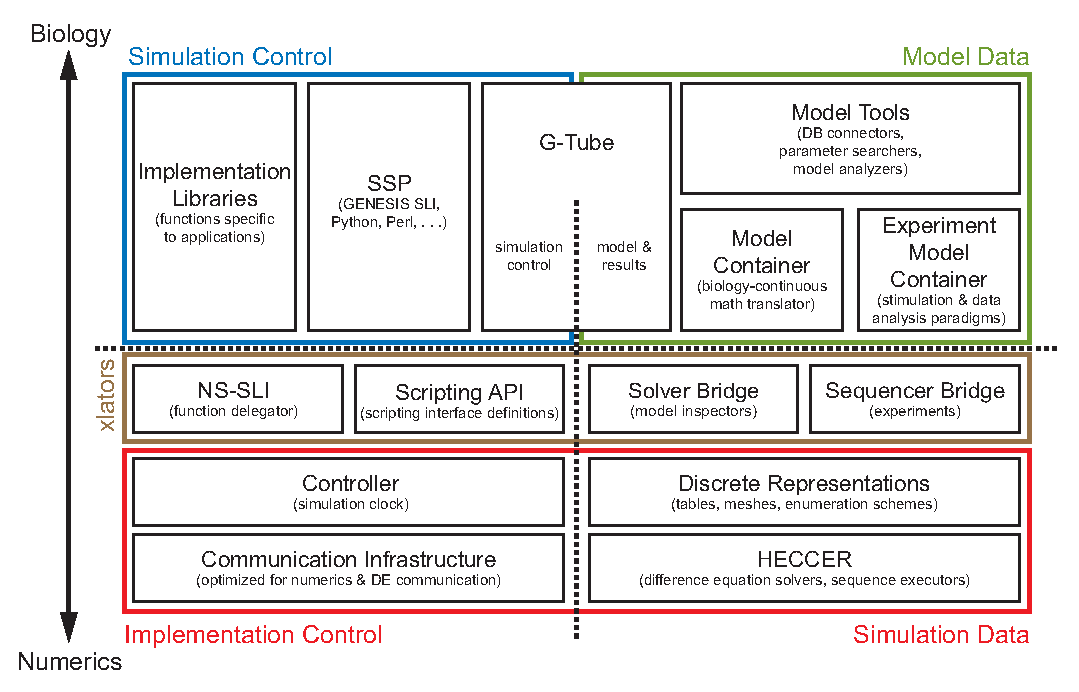
\includegraphics[width=4in]{figures/cbi-g3.eps}
%%  \includegraphics[scale=0.4]{figures/cbi-level2.png}
%\end{center}
%\caption{
%{\bf GENESIS 3.0.}
%The first implementation of the Computational Biology Initiative federated software architecture.
%}
%\label{fig:cbi_g3.eps}
%\end{figure}

%\clearpage


% Figure 1
\begin{figure}[ht]
\begin{center}
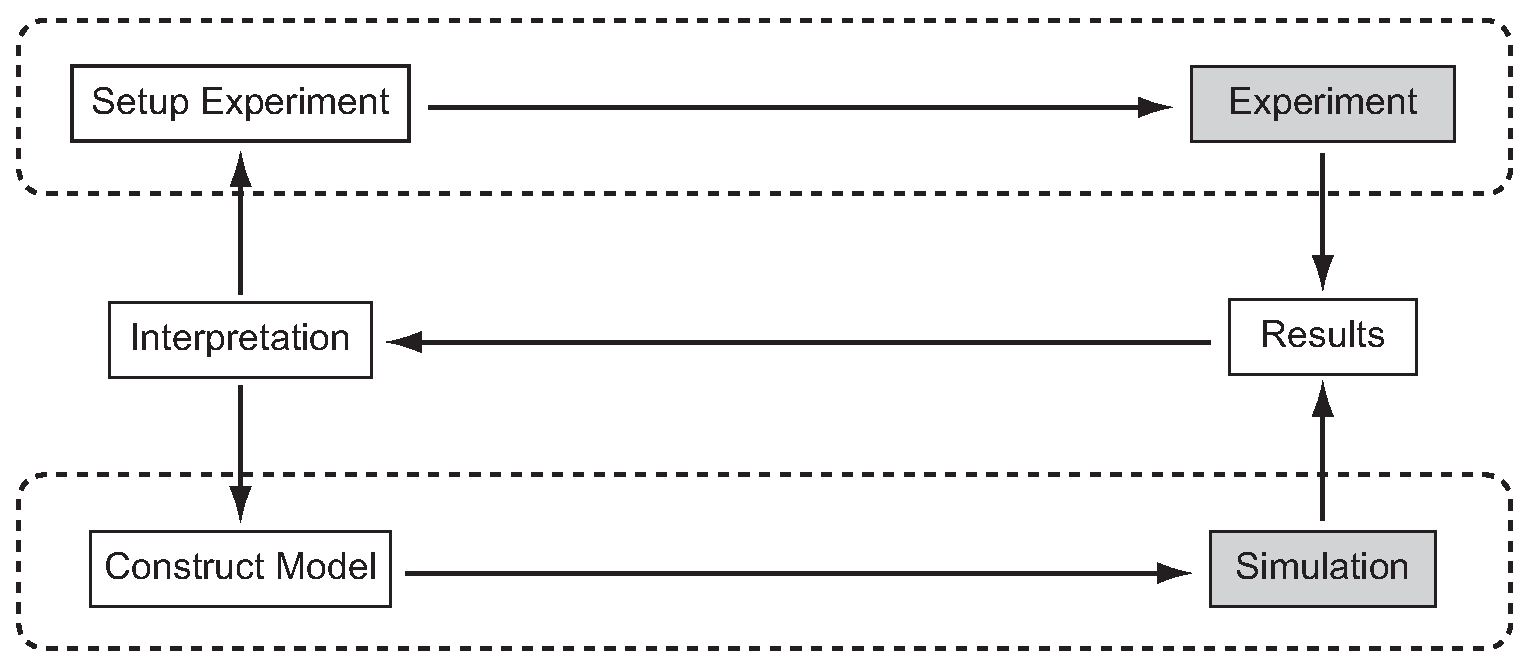
\includegraphics[width=4in]{figures/exp-sim.eps}
\end{center}
\caption{
{\bf Data flows in science.}
Conducting experiments and running simulations are two iterative processes indicated by the upper and lower dashed outlines. They are connected by an interposed feedback loop that uses the iterative interpretation of results to design new experimental setups and model constructions.
}
\label{fig:data-flows}
\end{figure}

\clearpage

% Figure 2
\begin{figure}[ht]
\begin{center}
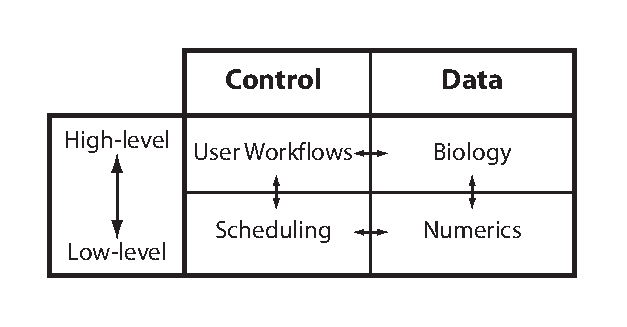
\includegraphics[width=4in]{figures/matrix.eps}
\end{center}
\caption{ {\bf Principle concerns.}  The four fundamental building
  blocks of a simulator are distinguished by separating (i) Data from
  control, and (ii) High level biological concepts from their
  mathematical implementation. In a federated architecture the only
  allowed interactions between modules are those indicated by the
  vertical and horizontal arrows. Diagonal interactions are forbidden
  as they ultimately lead to interactions that result in the creation
  of a monolithic software architecture.
}
\label{fig:data-control}
\end{figure}

\clearpage

% Figure 3
\begin{figure}[ht]
\begin{center}
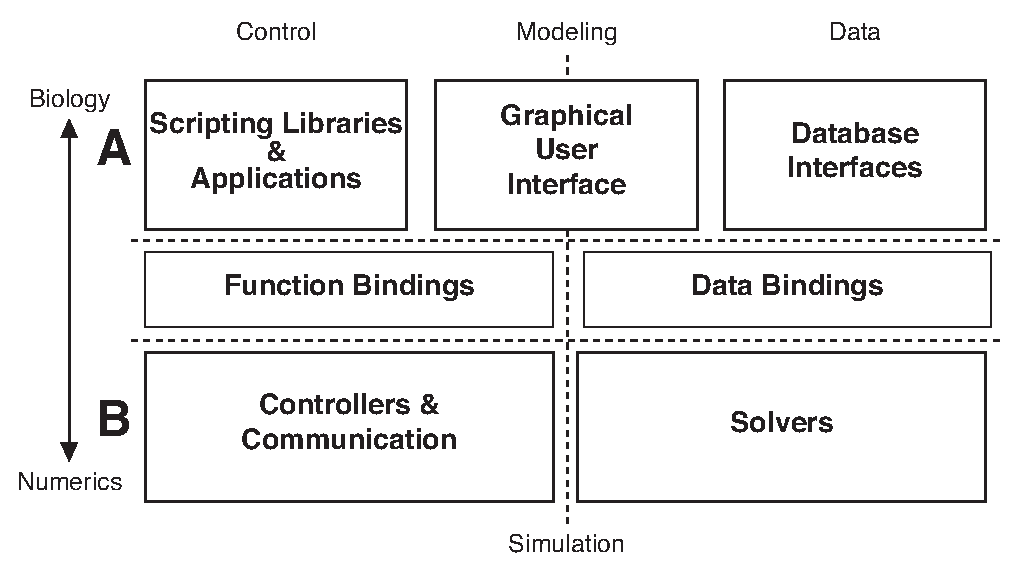
\includegraphics[width=4in]{figures/cbi-architecture-simple.eps}
\end{center}
\caption{
{\bf A federated software architecture.}
}
\label{fig:cbi-architecture-simple}
\end{figure}

\clearpage

% Figure 4
%\begin{figure}[ht]
%\begin{center}
%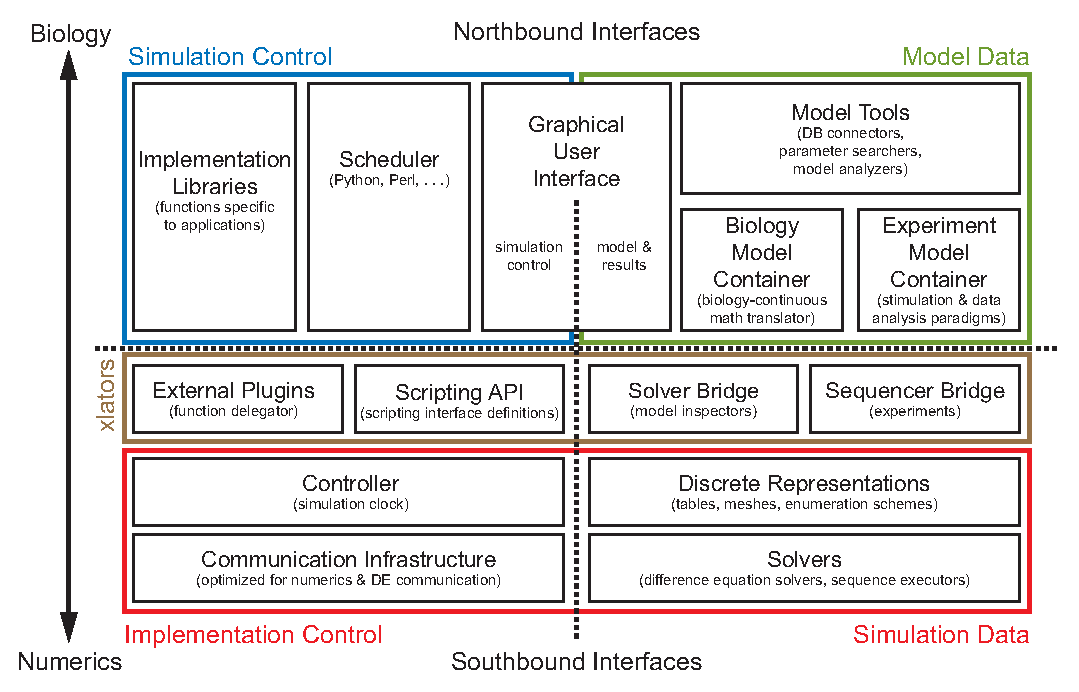
\includegraphics[width=4in]{figures/cbi-architecture-expanded.eps}
%\end{center}
%\caption{
%{\bf The Computational Biology Initiative federated software architecture.}
%}
%\label{fig:cbi-architecture-expanded}
%\end{figure}

%\section*{Tables}
%\begin{table}[!ht]
%\caption{
%\bf{Table title}}
%\begin{tabular}{|c|c|c|}
%table information
%\end{tabular}
%\begin{flushleft}Table caption
%\end{flushleft}
%\label{tab:label}
% \end{table}

%\begin{table}[!ht]
%\caption{
%\bf{Table title}}
%\begin{tabular}{|c|c|c|}
%%table information
%\end{tabular}
%\begin{flushleft}
%\end{flushleft}
%%\label{tab:cbi-codecounts}
%\end{table}

\end{document}
